\documentclass{report}

\usepackage{makeidx}
\usepackage{hyperref}
\usepackage{todonotes}
\usepackage{amsmath}
\usepackage{amssymb}
\usepackage{graphicx}
\usepackage{tikz}
\usepackage{acronym}
\usepackage[english]{babel}
\usepackage{blindtext}
\usepackage{acronym}
\usepackage{amsthm}
\newenvironment{bew}{\begin{proof}[Proof]}{\end{proof}}
\theoremstyle{definition}
\newtheorem{Satz}{Satz}[section]
\newtheorem{theorem}[Satz]{Theorem}
\newtheorem{ex}[Satz]{Example}
\newtheorem{cor}[Satz]{Corollary}
\newtheorem{algorithm}[Satz]{Algorithm}
\newtheorem{prop}[Satz]{Proposition}
\newtheorem{rem}[Satz]{Remark}
\newtheorem{defn}[Satz]{Definition}
\newtheorem{lem}[Satz]{Lemma}

\title{Leveraging Mathematical Structure in Software Synthesis (how to include part II?)}
\author{Andr\'{e}s Goens}
\begin{document}
\date{}

\maketitle
\tableofcontents
\clearpage
\section*{Acknowledgments}
Here will be the acknowledgments.


\chapter{Introduction}
Programming computers is notoriously difficult.
Indeed, people learning to program usually struggle, paradoxically, with the fact that the computer does precisely what they tell it to do. 
This is confusing not because a computer program is executed faithfully, but rather, because humans think at a very different level of abstraction.

It is certainly true that instructions in computer architectures are at a completely different level of abstraction than the instructions we give each other.
However, most programs are also not written at the level of the architecture.
Programming languages are designed with increasingly improving abstractions, to make it easier for programmers to express themselves.
Complementary to these efforts are compilers, which serve as bridge between the levels of abstraction.
Ideally, a compiler translates the abstract human-level expressions into efficient machine-level instructions.
While we have made significant progress, this task has proven to be dauntingly difficult.

Traditionally, we have put the resarch and effort into optimizing the execution of a single core.
Most of the progress of decades of research in programming language and compilers revolves around this single-core model.
In the last decade or two, however, with the multicore era, this challenge has increased dramatically.
Now we have to use and coordinate multiple cores, commonly with different capabilities.
The widespread programming language abstractions and compiler analyses of today are not well-suited to tackle this challenge.

\section{The Multicore Era}

On the hardware side, the last two decades have firmly established what we call the multicore era.
Modern computing systems are almost universally composed of multiple logical cores, and there is a clear trend of increasing both the number and the heterogeneity of these cores.
This increasing complexity brings about an increasing challenge in taming it.

\begin{figure}[h]
	\centering
   \resizebox{0.9\textwidth}{!}{\input{generated/moore.tex}}
   \caption{Chip trends as obtained from~\cite{microprocessordata}. The lines present the exponential growth prediction if considering data up until the year 2000.}
	\label{fig:multicore_era}
\end{figure}


%Multicore Era
Both the execution frequency and the closely intertwined single-core processing speed of computing systems increased exponentially up until the early 2000s (cf. Figure~\ref{fig:multicore_era}), an empirical fact observed by Gordon Moore in 1965~\cite{moore}.
Since the early 2000s, however, while tranistor size continue to decrease, the exponential frequency scaling has stopped (cf. Figure~\ref{fig:multicore_era}).
Individual and clever designs have continued to improve single-processor speed, albeit at a significantly slower rate.
Instead, most improvements in microchips in raw processing power have come from a paradigm switch.
Hardware designers resorted to develop multicores, microchips composed of multiple logical cores that can execute in parallel.
Additionally, since different use-cases benefit from different computing core architectures, the inclusion of multiple chips has paved the way for heterogeneity.
This has resulted in a multicore era of computing.

A programmer writing a piece of C code in the early 1970s would automatically benefit from the increasing processing speeds.
By recompiling her code for a processor $10 \times$ faster, she could very roughly expect her code also to run about $10 \times$ as fast.% Do I want to make this concrete (with Processor names?)
Nowadays thus, a programmer writing a piece of (sequential) C code in the early 2000s cannot expect anywhere near a $100$-fold increase in performance today when she uses a microchip with $100 \times$ the number of transistors.
At least not without fundamentally restructuring her code to exploit parallelism.
Contemportary systems aimed at performance almost ubiqutiously consist of multicore chips, in many cases heterogeneous, which tremendously increases the system complexity.
The trend is clear, the number of cores, heterogeneity and overall system complexity will only continue to increase.

%something about network-on-chip, emerging memories, and hierarchical topologies
As the number of cores in a chip keeps increasing, the importance of coordination and communication between the cores raises as well.
Memory latency and bandwidth has been a bottleneck for many clasess of applications for a while.
In the case of manycores, which are multicores where the number of cores goes over several dozens, even to hunderds or thousands, the on-chip memory subsystem becomes a central design point of the chip.
Systems based on \ac{NoC} technology become necessary, lest a single bus interconnect becomes the bottleneck of the system when thousands of cores want to communicate simmultaneously through it.

\begin{figure}[h]
	\centering
   \resizebox{0.5\textwidth}{!}{%Based on design by Marco Miani
%https://texample.net/media/tikz/examples/TEX/swan-wave-model.tex

\begin{tikzpicture}[scale=.9,every node/.style={minimum size=1cm},on grid]

    %slanting: production of a set of n 'laminae' to be piled up. N=number of grids.
    \begin{scope}[
            yshift=-83,every node/.append style={
            yslant=0.5,xslant=-1},yslant=0.5,xslant=-1
            ]
        \fill[white,fill opacity=0.6] (0,0) rectangle (5,5);
        \draw[black,dashed] (0,0) rectangle (5,5);%marking borders
        \pic [opacity=0.3] {fourmesh};
    \end{scope}
    	
    \begin{scope}[
    	yshift=0,every node/.append style={
    	    yslant=0.5,xslant=-1},yslant=0.5,xslant=-1
    	             ]
        \fill[white,fill opacity=0.6] (0,0) rectangle (5,5);
        \draw[black,very thick] (0,0) rectangle (5,5);%marking borders
        \pic {fourmesh};
    \end{scope}
    	
    \begin{scope}[
    	yshift=90,every node/.append style={
    	yslant=0.5,xslant=-1},yslant=0.5,xslant=-1
    	             ]
    	\fill[white,fill opacity=.9] (0,0) rectangle (5,5);
    	\draw[black,dashed] (0,0) rectangle (5,5);
        \pic [opacity=0.3] {fourmesh};
    \end{scope}
    	
    \begin{scope}[
    	yshift=170,every node/.append style={
    	    yslant=0.5,xslant=-1},yslant=0.5,xslant=-1
    	  ]
        \fill[white,fill opacity=0.6] (0,0) rectangle (5,5);
        \draw[black,dashed] (0,0) rectangle (5,5);
        \pic [opacity=0.3] {fourmesh};
    \end{scope}

    %putting arrows and labels:
    \draw[-latex,thick] (6.2,2.8) node[right]{Manycore}
         to[out=180,in=90] (3.5,2.3);

    \draw[-latex,thick](5.8,.3)node[right, align=center]{Optical \\ Interconnect}
        to[out=180,in=90] (3.3,-0.8);

    \draw[-latex,thick](5.9,7.5)node[right,align=center]{Wireless \\inter-board \\ links}
        to[out=180,in=0] (3.6,7.0);
\end{tikzpicture}}
   \caption{The HAEC architecture~\cite{HAEC} has multiple levels of hierarchy: on-chip, intra-board (optical links) and inter-board (wireless).} 
	\label{fig:haec}
\end{figure}

In fact, for a multitude of reasons, manycores are commonly designed in a hierarchical fashion.
Smaller clusters of cores locally interconnected communicate between each other and off-chip via a larger \ac{NoC}.
These clusters and systems are usually heterogeneous as well, like the Karlay MPPA3 Coolidge, with includes accelerators for cryptography and secure cores, alongside general purpose cores.
Some systems even propose multiple layers of hierarchy, like the three layers of the HAEC topology~\cite{HAEC}, depicted in Figure~\ref{fig:haec}.
This is a proposed 3D stacked system with multiple boards each with multiple chips, not a single chip with this complex interconnect.
However, this design could allow for very low latencies, such that challenges of programming it are comparable to those of programming such a topology in an on-chip memory subsystem.
What happens if the mulicores in this system are similar to the Karlay MPPA3 Coolidge? This would yield more than $5000$ heterogeneous cores connected at five levels of hierarchy in different topologies.
More generally, complex topologies with possibly multi-level hierachies, add an additional layer of complexity to modern manycore systems besides heterogeneity and concurrency.

\section{Programming Multicores}

As already mentioned, programming is notoriously difficult since it translates from the level of abstraction of human interactions to the instructions of a computing system.
The multicore era greatly aggravates this already difficult problem.
We speak of a software productivity gap~\cite{castrillon2014thesis,ecker2009hardware}\index{software productivity gap}. 
The productivity of developers cannot keep up with the pace of developments in hardware.

When programming multicore systems, abstractions that proved very useful for programming single-cores become inadaquate.
An universal concept in programming is that of repeating an action multiple times, or looping. 
This perfectly exemplifies the differences in abstractions and how they become inadequate for multicore systems.

For example, consider the task of iterating through a bunch of pictures and determining which of them contain cats.
For instructing a human, we can probably say something like ``look through those pictures and sort out the ones have cats''.
A modern x86 chip, on the other hand, would understand something closer to this:

\begin{minted}{Nasm}
LBB0_1:                                 
	cmp	dword ptr [rbp - 56], 10
	jge	LBB0_4
	mov	edi, dword ptr [rbp - 56]
	call	_read_file
	mov	qword ptr [rbp - 64], rax
	mov	rdi, qword ptr [rbp - 64]
	call	_contains_cats
	movsxd	rcx, dword ptr [rbp - 56]
	mov	dword ptr [rbp + 4*rcx - 48], eax
	mov	eax, dword ptr [rbp - 56]
	add	eax, 1
	mov	dword ptr [rbp - 56], eax
	jmp	LBB0_1
LBB0_4:
	mov	eax, dword ptr [rbp - 52]
	mov	rcx, qword ptr [rip + ___stack_chk_guard@GOTPCREL]
	mov	rcx, qword ptr [rcx]
	mov	rdx, qword ptr [rbp - 8]
	cmp	rcx, rdx
	mov	dword ptr [rbp - 68], eax 
	jne	LBB0_6
\end{minted}

This snippet is a very oversimplified version of the task, but it serves to make the point.
Where we abstractly tell a human to look through the pictures and they undestand them as a whole set, interpreting themselves how to go through the set.
On the other hand, we instruct the machine to iterate through them by a series of very fine grained commands.
We need to set certain registers to contain the right memory addresses, before calling an instruction to operate on them.
Here we then call external functions that do the reading and cat identification.
To then loop through the pictures here, simplified, we repeat this reading and indetifying by jumping to a previous point in the sequence of instructions.
Even this x86 assembly snippet is already an abstraction, not only because it uses human-readable mnemonics for the instructions, but more so because it also abstracts away the concrete memory addresses.
In practice, however, almost no one would write this assembly code. Instead, they could write something closer to this (equivalent) C snippet:
\begin{minted}{C}
for(i = 0; i < N; i++){
    char *f;
    f = read_file(i);
    results[i] = contains_cats(f); 
}
\end{minted}

Notice how the register management and several other low-level details are abstracted away.
The end of the loop is very clear to read, as we know when we have reached the final picture.
We can certainly say this is at a level of abstraction between the human and machine instructions contrasted above.
However, the very widespread \texttt{for} instruction we used here also has the inherently sequential semantics exhibited by the machine code above.
The semantics of the for loop are that the loop body will execute completely.
After each iteration of the body, the increment expression is executed (usually incrementing the iteration variable), and the condition is evaluated, deciding wether to continue iterating.
Indeed, in the two (equivalent) snippets above, we don't know how the functions\texttt{read\_file} and \texttt{contains\_cats} work.
Do they have an inner state, or side effects?
We don't know if we can call \texttt{read\_file} in a different order, or multiple times in parallel.
Perhaps it is internally keeping a single reference to the iterator of the image files and doing so would break the logic.
The \texttt{for} instruction is very useful to abstract away the logic of registers and instruction jumps, but not a useful abstraction for expressing concurrency.
A similar construct exists in functional programming, \texttt{map}\index{\texttt{map} function}, which generally does not have this implicit sequential semantics.
The \texttt{map} instruction is what is called a higher-order function\index{higher-order function}, taking a function as an argument and applying it to a list or any iterable object, in general.
The same cat-identifying snippet, in Haskell, can be written as follows:
\begin{minted}{Haskell}
result = map (contains_cats . read_file) pictures
\end{minted}

While the language separates statfull and stateless computation, allowing a great analysis of concurrency, there are reasons why Haskell is not the most widespread language for embedded systems.
For example, garbage collection makes execution times very unpredictable.
Similarly, the lazyness of the language adds a performance penalty to large complex computations.
Compiling Haskell code to an efficient single-core execution is significantly more challenging than with the C code.
The lazyness also makes it difficult to reason about time in the computation.
This is crucial in some application domains, like \ac{CPS}, where the systems interact with their environment.
The \texttt{map} abstraction as implemented in Haskell is thus not well-suited to the domain of \ac{CPS}.
In general, we are faced with trade-offs between abstract expressability and translatability to an efficient execution.
At its core, the challenge is about choosing the right models and corresponding abstractions for a particular domain.

\section{Software Synthesis}

Models play different roles in science and engineering.
E.A. Lee explains this well in~\cite{lee2017plato}.
He argues that scientist adapt their models to fit experiments in the world, while engineers adapt designs in the world to fit their models.
Indeed, for some fundamental principles of computation, like $\lambda$-calculus, are discovered instead of invented~\cite{wadler2015propositions}.
Those might fit in the first paradigm, giving computer science a justification for its name.
In the case of programming multicore systems, however, the problem is clearly in the second realm: we need to engineer good models~\cite{lee2006problem}.
No serious argument can be made for languages like C or Haskell, nor the x86 instruction-set; They were invented, not discovered.

There are different ways of finding and exploiting the right models for programming multicores.
It is unlikely that there is a single right model for this.
Different models are differently suitable for different use-cases. 
For example, applicative functors in functional programming~\cite{marlow2014haxl} seem to be a great model for expressing \acs{I/O} concurrency in microservice-based systems.
%We will discuss this example in Chapter~\ref{chap}.
As mentioned before, however, Haskell and its underlying model are not a great fit for \ac{CPS}.

For \ac{CPS} and, embedded systems in general, there is a family of methods called software synthesis~\cite{ritz1992softwaresynthesis,abbott1993softwaresynthesis,lin1998softwaresynthesis,bhartacharyya2000softwaresynthesis,pino1995softwaresynthesis,bhattacharyya2012softwaresynthesis}\index{software synthesis}.
It is a family of methods devised precisely to help with the burden of fully exploiting the capabilities of modern multicores.
Inspired by hardware design flows, it aims to bridge the ensuing (software) productivity gap by integrating knowledge of the application and target multicore architecture into the compilation process.
At the core of these methods lies a shift in the programming model.
Instead of the de-facto sequential, shared-memory model, programmers express the code in diverse \acp{MoC}.
This makes the underlying model explicit, not implicit as is the case in most programming languages.

These models expose the structure of the computation in ways that permit a compiler to reason about its parallel execution, even in the prescence of heterogeneous hardware.
Aided by abstract models of the target archicecture, we can design compilers for multicore systems that devise execution strategies specialized to the target architecture and applications.
Depending on the flow, the target archicecture can be implicit in the methodology~\cite{ritz1992softwaresynthesis} or be an explicit input to the flow~\cite{maps}
This can be realized for example by finding efficient mappings, i.e. allocations of computational and communication resources to the different parts of an application.

As mentioned above, the central principle behind software synthesis is the underlying model of computation. 
Some approaches~\cite{lin1998softwaresynthesis} use very general models, like Petri Nets~\cite{petri1962nets}, while others~\cite{ritz1992softwaresynthesis} very constrained models like \acp{SDF}~\cite{lee1987sdf}.
Most allow for multiple models~\cite{bhartacharyya2000softwaresynthesis,pino1995softwaresynthesis,bhattacharyya2012softwaresynthesis}, generally dataflow models.
Making the model explicit just makes it easier to see the trade-off between expressability and translatability to an efficient execution.
The advantage of models like Petri-Nets is that they are very general and can express virtually any computation.
On the other hand, very constrained models, like \ac{SDF} provide behavioral guarantees that permit several optimization, like static schedules and channel bounds~\cite{Parks:M95/105}.

Several more modern flows~\cite{thiele2007DOL,maps,pimentel2006systematic,kangas2006uml} have settled at the \ac{KPN} model.
Originally meant as denotational semantics for parallelism~\cite{kahn74}, the model has been shown to be compatible with the dataflow~\cite{lee1995dataflow}.
Kahn Process Networks are provably deterministic~\cite{kahn74}, which is not the case for other models, e.g. Petri Nets.
In a canonical sense, \acp{KPN} are more general than most dataflow models, and represent the most general deterministic dataflow model of computation~\cite{lee_matsikoudis_semantics}.
In this thesis we will focus on a software synthesis flow~\cite{maps,castrillon2014thesis} based on \ac{KPN}.
Figure~\ref{fig:software_synthesis_flows} shows the general structure of the flow and the four main abstractions as we identify them for our analysis~\cite{goens_mcsoc16}.
Chapter~\ref{chap} will review these abstractions, including the models of computation above, and their relationships.

\begin{figure}[h]
	\centering
   \resizebox{0.75\textwidth}{!}{% Define block styles
\tikzstyle{flow} = [rectangle, rounded corners, draw, fill=green!20, %legend: possible "IP leak"
    text width=7em, text centered, minimum height=4em]
\tikzstyle{abstract} = [rectangle, draw, fill=blue!20, 
    text width=7em, text centered, rounded corners, minimum height=4em]

\begin{tikzpicture}[node distance = 4em]
    %nodes
    \node [abstract ] (moc) {Application (Model of Computation)};
    \node [abstract, below=of moc] (exec) {Execution};
    \node [flow, right=of moc ] (kpn) {Kahn Process Networks (KPN)};
    \node [flow, right=of exec] (traces) {KPN Traces (Histories)};
    \node [abstract, right=of kpn ] (arch) {Architecture};
    \node [abstract, right=of traces] (decisions) {Decisions};
    \node [flow, right=of arch] (archgraph) {Architecture graphs, ad-hoc models};
    \node [flow, right=of decisions] (mappings) {Mappings};
    \node [below=of traces] (todo) {TODO: improve this figure! (based on MCSOC'16)};


\end{tikzpicture}
}
   \caption{The four main abstractions in Software Synthesis in the Example of a \acs{KPN}-based flow.} 
	\label{fig:software_synthesis_flows}
\end{figure}

\section{Contribution}

In this thesis we seek to improve the tools we use for understanding and tackling the problems we've introduced. 
We work around in a model-based perspective and consider the trade-off we've introduced, between abstract expressability and translatability to an efficient execution
To consider this we tackle the problem from both sides: the models and the compilers, in a very general sense, that translate to an efficient execution.
The main idea behind this thesis is that the underlying models endow the problem with structure.
We can then identify this structure (mathematically) and leverage it to improve our solutions.
Again there are two ways of doing this: 
\begin{enumerate}
\item by taking a concrete flow and improving it leveraging its own structure, or
\item by changing the underlying model in a way that improves the balance in some way in the trade-off above.
\end{enumerate}
These make the two parts of this thesis.


The first part focuses on software synthesis in the domain of \acp{CPS} and generally embedded systems.
While some of the difficulties are general of all computing systems, the largest challenges are usually specific to an application domain.
This thesis focuses on one such domain, of \acp{CPS} and other high-performance embedded systems running on \acp{MPSoC}.
In particular, we focus on a concrete software synthesis flow~\cite{maps,castrillon2014thesis} based on \acp{KPN} (cf. Fig.~\ref{fig:software_synthesis_flows}). Chapter~\ref{chap:background} introduces this flow and the corresponding background.


% Exploiting Structure in Dataflow Software Synthesis: Part I
As described in Figure~\ref{fig:software_synthesis_flows}, the software synthesis process is centered around multiple abstractions.
These can be seen as formal constructs modeling the application and architectures, as well as decisions of the execution of the former on the latter, like mappings.
They are all rich in (mathematical) structure.
Architectures for example, even heterogeneous ones, exhibit a great deal of symmetry.
Similarly, the space of mappings has locality properties, where some mappings are similar whereas others are to others . Chapter~\ref{chap:structures} describes these structures.
In this thesis we aim to identify and exploit these structures in different ways.

Chapter~\ref{chap:compile-time} explores compile-time applications of the identified structures.
For example, it shows how we can use symmetries in \ac{DSE} for pruning the design space and discusses the role of locality in mapping algorithms.
Chapter~\ref{chap:mapping_other_applications}, on the other hand, explores other applications of the structures.
It shows how symmetries can also be leveraged at runtime in so-called hybrid mapping strategies.
It also discusses memory, which is traditionally neglected in mapping approaches.
\todo{The structure of the applications feels weird: can I change it?}
In Chapter~\ref{chap:mapping_conclusions} we discuss the conclusions we can make from exploring this mapping flow,
and we also discuss related work to this part in Chapter~\ref{chap:related_mappings}.

The second part of this thesis goes beyond the discussed \ac{KPN}-based flow.
Instead of the structure emerging from a concrete model, i considers the underlying models themselves.
While Software Synthesis refers to a family of methods, each concrete method has a corresponding choice of abstractions it uses.
This translates to the programming language abstractions and semantics striving for expressive idioms for programmers that permit the compiler to analyze them and execute them efficiently.
Thus, instead of exploiting the structure of the given abstractions, in the second part of this thesis we explore ways in which we can improve upon software synthesis methods by changing the structure we use: be it the semantics of the model of computation, implicit language structures or even the benchmarks we evaluate to asses our methods.

In Chapter~\ref{chap:mocs} we start with a more systematic overview of \acfp{MoC}.
We see how understanding the models and their relationships pays off by finding and exploiting a gap in the semantics between \ac{KPN} and languages that usually implement this model using blocking-reads semantics.
Expanding on the overview of \acp{MoC}, we consider the requirements of the domain of \acp{CPS}.
From these considerations we discuss a novel model, Reactors, and how it can be used in different domains like automotive and telecommunications.
In Chapter~\ref{chap:language} we go beyond the realm of \acp{CPS} and discuss how the principles of dataflow and language-based transformations can be exploited in a different domain, this time in a different domain of microservice-oriented systems. We discuss two distinct ways to exploit language-level abstractions in this domain.
Finally, in Chapter~\ref{chap:benchmarknig} we turn our attention to a seemingly orthogonal aspect: Benchmarking.
In order to asses the performance of any method or flow, we require benchmarks.
However, benchmarks are scarce and of very diverse levels of quality.
Nevertheless, we can exploit structure again to combat this problem: instead of the structure of the models and architectures, we consider the structure of the applications and their code.
We show how we can achieve this both with hand-made models, and using machine learning to learn the structure of the applications.

We discuss related work to the different aspects of this second part in Chapter~\ref{chap:related_semantics}.
We then expand our conclusions from the \ac{KPN} flow to consider these additional aspects, concluding the thesis in Chapter~\ref{chap:conlusion.}
\todo{Add a discussion of the motivation to constraint in the right way. Do I have a good example? (GOTO?), cite~\cite{tasharofi2013scala}} 

\subsection{A Note on Originality}

This thesis presents the fruits of over half a decade of research on the subjects presented.
Research, especially in an interdisciplinary approach like presented here, is much more fruitful when collaborative.
In the case of joint work, I have made an effort to focus only on my own contributions in this thesis, whenever possible.
I have also taken care to describe the work of my colleagues as theirs, when I have included it as an indispensable requirement to understand my own work.
However,  many if not most of these ideas in these thesis are the result of joint work and cannot be credited to a single person.
In those cases I have also taken care to describe the work as joint and mention other co-authors.
If in doubt, any idea or result that I have included here which has already been published elsewhere is also due to my coauthors.

%\begin{figure}[h]
%	\centering
%   \resizebox{0.55\textwidth}{!}{\begin{tikzpicture}
\draw (0,0) rectangle (5,5);
\draw (2.5,2.5) node {Placeholder};
\end{tikzpicture}
}
%	\caption{A placeholder picture.}
%	\label{fig:placeholder}
%\end{figure}
%
%\end{figure}
%\begin{figure}[h]
%	\centering
%   \resizebox{0.55\textwidth}{!}{\input{generated/placeholder_plot.tex}}
%	\caption{Placeholder plot.} %something like: https://www.karlrupp.net/wp-content/uploads/2015/06/40-years-processor-trend.png
%	\label{fig:placeholder_plot}
%\end{figure}

%A placeholder reference\cite{goens_multiprog18}.
%\begin{figure}[h]
%	\centering
%   \resizebox{0.55\textwidth}{!}{\input{figures/placeholder_flow.tex}}
%	\caption{A placeholder flow.}
%	\label{fig:placeholder_flow}
%\end{figure}



\part{Dataflow-based Software Synthesis(?)}
In this firt part of the thesis we will consider the software synthesis process as has been traditionally been studied, considering its mathematical structures and proposing improvemnts that do not fundamentally change the setting. The second part will go beyond this model and propose novel directions to adapt the model itself.

\chapter{Mapping KPNs to Heterogenous MPSoCs}
Software synthesis refers to a series of related methods, with the common goal of efficiently deploying software on a specific hardware architecture. While the aim of this thesis is to analyze structures and present methods that are general to software synthesis as a whole, in practice we will always work with concrete design flows. In this chapter we will introduce the concepts behind software synthesis and mappings in a concrete such flow, mapping KPN applications onto heterogeneous hardware. The flow can be seen in Figure~\ref{fig:sofware_synthesis_flow}, and is presented in detail in~\cite{castrillon_phd}.

As is general in Software Synthesis, the applications to be axecuted are represented with an abstract representation linked with a model of computation, Kahn Process Networks (KPNs). Similarly, the target archtiecture is assumed to be known at compile-time, and is models via an abstract architecture model. The KPN model has a property that allows to capture the abstract execution behavior in a trace that is independent of the execution target. Combining these application and architecture models, and using an execution trace, a simulation can be used to estimate the performance of a mapping - an assignment of physical execution and communication resources on the target architecture to the logical (abstract) components of the KPN application. In an iterative process, this estimations can be leveraged to determine a near-optimal mapping subject to objective goals (e.g. execution time, energy conspmution). Finally, a compiler can lower the KPN application to an executable that uses the selected mapping.

The rest of this chapter will explore the various models refered to in this flow, with precise mathematical definitions and a discussion of common design choices and goals in this flow.

\section{Kahn Process Networks}
\Blindtext[2]

\section{Models of Heterogeneous Architectures}
\Blindtext[2]
Briefly discuss MoA paper (Pelcat et al).

\section{Traces}
\Blindtext[2]


\section{Mappings}
\Blindtext[2]

\section{Background}
At the basis of software synthesis are concurrent models of computation. The process derives an efficient execution to a concrete architecture from a computation expressed in an abstract model.
In order to understand software synthesis thus, we first need to understand the underlying models of computation.
Closely related to these concurrent models of computation are execution traces, which capture a concrete execution for some input.
However, going from such abstract models to a concrete execution also requires an understanding of the target hardware architecture.
The relationship between the two can be captured in a mapping.
This chapter considers all of these aspects with their corresponding models, and the relationship between them.
It is the central piece of background theory required for the methods presented in this thesis.

\subsection{Models of Computation}
\label{sec:mocs}

In his seminal paper~\cite{turing1936computable} in 1936, Alan Turing proposed a ``computing machine''\footnote{now known as Turing machine}.   
While his machine was motivated by a person doing computations, he intended to capture the very notion of compatibility by it: namely what it is possible to compute at all.
He was modeling computation.
Two additional such models of computation existed at the time, the $\lambda$-calculus as proposed by Alonzo Church that same year~\cite{church1936unsolvable}, and the concept of general recursive functions due to Herbrand and Gödel, developed by Kleene~\cite{kleene1936recursive}.
These three equivalent models~\cite{turing1937comuptability} were the original models of computation.
They are equivalent in the sense that they define the same notion of what is computable.
However, they are not equivalent in the number of steps necessary for computing something.
To an extent these models were not concerned with how to (efficiently) compute something, but rather, \emph{what} we can compute and what not.

With the revolution of digital computers, the interest increasingly shifted to care about \emph{how} we can compute.
In 1972 Karp\cite{karp1972reducibility} kickstarted the field of computational complexity by identifying many problems that were equivalently difficult to compute, the class of NP-complete problems.
Computational complexity relies on the fact that the asymptotic behavior of the number of steps of an algorithm, as a function of the input (size), is invariant when changing between these models of computation.
Around the same time, in 1970, Dana Scott proposed a mathematical theory of computation~\cite{scott1970} based on what are now called (Scott) domains\footnote{sometimes also called algebraic semilattice} and the Scott-topology. 
Two ideas are central in Scott's formalization. The first is a method for capturing \emph{partial} computations, i.e. computations that have advanced but not finished yet.
The second idea is that of modeling a computation as a continuous function between such domains, where a properly notion of continuity (in the Scott topology) models causality in the computation.
Scott's semantics allowed to capture the process of a computation, but not the internals, which are abstracted away by the function. 

The question of \emph{how} we compute can be modeled in different ways by complexity asymptotics or partial computations in the Scott formalism, but some aspects are still left unmodeled.
A significant such aspect not taken into account by these models is \emph{where} we are computing.
The theory of distributed computation was growing, with models like Petri Nets~\cite{petri1962nets} or seminal work like Lamport's on clocks and ordering of events~\cite{Lamport1978time}.
These models deal with properties of a computing system that has physically separate parts which split and distribute the computational load.
However, the focus of the models is the system doing the computation, not the computation itself.

In this thesis we are mostly interested in concurrent models of computation. 
Such models abstract away the (distributed) computing system and focus on the computation itself. 
They consider and express concurrency in the computation, which can be exploited for parallel or asynchronous execution.
The rest of this section will survey some of the most important concurrent models of computation, before moving on to architectures, traces and mappings.


\begin{figure}[h]
	\centering
   \resizebox{0.55\textwidth}{!}{\begin{tikzpicture}%[fill opacity=0.3]
%circles
\node[ellipse, fill=green!20, minimum width = 9cm,minimum height = 5cm,draw] (ddf) at (0,3) {};
\node[ellipse, fill=green!60, minimum width = 6.2cm,minimum height = 4.5cm,draw] (kpn) at (1,3) {};
\node[ellipse, fill=green!50, minimum width = 5.5cm,minimum height = 4.0cm,draw] (kmq) at (1,2.8) {};
\node[ellipse, fill=green!70, minimum width = 4.8cm,minimum height = 3.5cm,draw] (csdf) at (1,2.6) {};
\node[ellipse, fill=green!30, minimum width = 3cm,minimum height = 3cm,draw] (sdf) at (1.5,2.5) {SDF};
\node[ellipse, fill=green!40, minimum width = 1.0cm,minimum height = 1.0cm,draw] (hsdf) at (1.5,3.4) {HSDF};

%labels
\node (lbl-ddf) at (-3,3) {DDF};
%\node (lbl-sdf) at (0,1.5) {SDF};
%\node (lbl-hsdf) at (0,0) {HSDF};
\node (lbl-kmq) at (1,4.5) {KMQ};
\node (lbl-sadf) at (-0.6,2.5) {CSDF};
\node (lbl-kpn) at (1,5.0) {KPN};
  
\end{tikzpicture}
}
	\caption{Relationships between different dataflow models of computation.}
	\label{fig:dataflow_mocs}
\end{figure}

\subsection{Partial Computation: Scott Domains}


A Domain is a particular type of \ac{poset} ... 

For example ...


Scott's computation model implicitly assumed a sequential computation and Scott-continuous functions are a powerful method for describing partial sequential computations.
Can we also use this model to describe parallel computation?
Gilles Kahn did precisely this, four years after Scott published his mathematical theory of computation. 
He used the formalism of Scott to define a model of parallel computation, based on what he coined as process networks, now known as Kahn Process Networks.

The basic idea to generalize the Scott theory of computation is simple



\subsection{Concurrent Computation: Kahn Process Networks}
\Blindtext[10]


\subsection{Dataflow Models of Computation}
Dennis~\cite{dennis1974first,dennis1986data}
\cite{Parks:M95/105}
Dataflow process networks~\cite{lee1995dataflow,lee_matsikoudis_semantics}
CSDF~\cite{bilsen1996cycle}
SADF~\cite{theelen2006scenario}
\cite{lee1987sdf}
\Blindtext[10]

\subsection{Execution Traces}
See~\cite{mazurkiewicz1995introduction} in~\cite{diekert1995book}
\Blindtext[10]

\subsection{Architecture Models}
\cite{pelcat2015models}.
\Blindtext[10]

\subsection{The Mapping Problem}
\cite{singh2013mapping}
A lot more...
\Blindtext[10]
\subsection{Limits of the Model}
\Blindtext[10]


\section{Simulating Mappings}
Simulations are extremely important for analyzing an application's performance, or more generally, its behavior.
As described in Section~\ref{sec:arch_models}, there are multiple levels of detail in which to model and, consequently, simulate, an architecture and its execution.
For investigating the mapping problem in software synthesis, higher-level simulations are preferable for multiple reasons.
First and foremost, higher-level simulations are faster.
If a meta-heuristic iteratively evaluates dozens, hundreds or even thousands of mappings to find a near-optimal one, it greatly benefits from the fast evaluation time associated with a higher-level simulation.

Higher levels of abstraction come with a trade-off, accuracy of the simulation suffers in exchange for the simpler models and faster simulation times.
Let $\tilde \Theta$ be the approximation of $\Theta$ from the simulation. A loss in accuracy means that $| \Theta(m) - \tilde \Theta(m)|$ becomes larger.
However, depending on the use-case and mapping objective $\Theta$, this loss in simulation accuracy might not necessarily affect the quality software synthesis results.
Suppose that the objective $\Theta$ represents execution time or energy consumption, and the goal of the software synthesis is just a best-effort minimization of $\Theta$ (with no additional constraints, i.e. $C \equiv \operatorname{True}$).
Then the accuracy of the simulation is not important, only its fidelity.
If $\Theta(m_1) < \Theta(m_2)$ we want the result of the simulation to reflect this, $\tilde \Theta(m_1) < \tilde \Theta(m_2)$.
As long as this is the case, we don't care about the actual value of $| \Theta(m_i) - \tilde \Theta(m_i)|$, since in this case the exploration will still find the minimum.
The fidelity of the simulation is a measure of how often this is true.
On the other hand, if the application is a real-time application, then the truth value of $C$ will depend on the accuracy of the simulation.
Here, the accuracy of the simulation is much more important.

This chapter describes the simulation aspects which pertain the models of computation and the practical tooling we will use.
Nuanced simulation details and advanced techniques are beyond the scope of this thesis.

\subsection{Simulating the Execution of Kahn Process Networks}

The behavior of a system plays a central role in simulation. A deterministic model should yield deterministic simulation results.
Non-determinism, when present, should also be captured by the models and reflected by the simulations.

The behavior of systems is commonly captured in execution traces, which simply record the behavior of different entities (e.g. processes or actors) at different timepoints.
This can be formally captured in a monoid structure of (Mazurkiewicz) traces or, equivalently, histories~\cite{diekert1995book}.
Traces are useful to understand the behavior of systems~\cite{vampir} and are common in many domains.
However, for systems that are non-deterministic, (by definition) the behavior of the system does not only depend on the input.
This can make designing~\cite{lee2006problem} and debugging~\cite{murillo_debugging} particularly difficult.
In cyber-physical-sytems or, more generally, reactive systems in the sense of Harel and Pnueli~\cite{harel_pnueli_reactive}, input from the physical world might come in a non-deterministic fashion.
The problem of capturing the behavior of such a system is even more complex when the system is distributed~\cite{shaver_phdthesis}. 

Kahn Process Networks are deterministic, as are all the dataflow models that can be embedded as KPNs.
This means that the behavior of a KPN application depends only on the input to the network.
In particular, it does not on the mapping and scheduling or related execution details.
Thus, their behavior can be captured by a (Mazurkiewicz) trace.
This permits to re-create their behavior in a fashion that is independent of the mapping~\cite{find_proper_references}.
By ``replaying'' the trace, i.e. simulating the execution of a process for every input in the trace, a discrete-event simulator can successfully simulate the execution of a KPN, since the token sequence is guaranteed to be identical given identical inputs.
In particular, this allows us to do design-space exploration.

A discrete-event simulation of a KPN application thus requires behavior traces. It also needs to model the execution and communication times.
Modeling execution times from a trace is simple, with a crucial assumption: if the execution times for a trace event only depend on the PE type.
This assumption won't hold always hold, e.g. when the instruction cache is flushed due to scheduling decisions, or due to unpredictability from the \ac{OS}.
Note that data caches are modeled as part of the communication between processes.
However, in most cases this assumption is a good approximation, it is normal to expect that the same code executing on the same data and the same \ac{ISA} will usually require the same amount of time.

Modeling communication is more complicated, as it depends on the memory subsystem. In general, the communication costs of sending a KPN token depend on multiple factors, like the size of the token, contention in the memory subsystem (and correspondingly methods of arbitration, routing in the case of a \ac{NoC}, etc), or the API and protocol being used.
For the simulations in this thesis, we use a model based on annotations of the architecture graph $A$. These annotations are functions that calculate the time cost of communicating data, as a function of its size.
In this way, we model both the latency and bandwidth of the communication.
We use a split-cost communication model to assign costs to sending and receiving data~\cite{odendahl2013split}.
This separation can be used to simulate based on traces, as described above, since we can then compute the cost of communication for both the sending and receiving processes.

When dealing with \ac{NoC}-based architectures, this model is not as accurate.
Communication over a \ac{NoC} depends also on the routers and links along the path, including the routing algorithms.
We extended the split-cost communication model to account for these issues in~\cite{menard_norcas16}.
The idea is to add a third term to account for the network, in addition to the consumer and producer costs. 
This third term can account for the routing and the topology of the network while maintaining an analytic model which is cheap to evaluate in a high-level simulation.

Simulation is essential for software synthesis, yet it is not the focus of this thesis. As such, we will only discuss the main idea behind the analytic models and their relationship to a fast simulation of \ac{NoC}-based architectures.
The main contribution of~\cite{menard_norcas16}, with a concrete model for the Tomahawk~2 architecture~\cite{tomahawk2} and the corresponding evaluation comparing to the SystemC-based simulator Noxim~\cite{noxim} are due to my coauthors and beyond the scope of this thesis.

\subsection{Mocasin}

In this thesis we will use mocasin, a tool for the Model-of-Computation-based Analysis and Simulation of applications~\cite{menard_rapido21}.
This tool, formerly known as pykpn~\cite{goens_mcsoc18}, has been developed as part of a collaborative effort between multiple researchers at the Chair for Compiler Construction at TU Dresden.
While the tool itself is a joint contribution with the coauthors of~\cite{menard_rapido21}, many concepts introduced in this thesis have been implemented and tested using mocasin.
As such, this section will explain the tool in-depth, to enable the description of the different implementations of contributions from this thesis implemented in mocasin.

\begin{figure}[h]
	\centering
   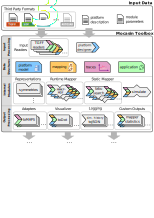
\includegraphics[width=0.95\textwidth]{figures/mocasin.pdf}
	\caption{The mocasin architecture. Adapted from \cite{menard_rapido21} (Figure~2).}
	\label{fig:mocasin_kpn_simulation}
\end{figure}


Figure~\ref{fig:mocasin_kpn_simulation} depicts the basic flow of simulating KPN applications in mocasin.
In general, simulating a KPN requires four inputs, as explained in Section~\ref{sec:mappings_background}: the KPN graph, a platform description, execution traces and a mapping.
Instead of a concrete trace, mocasin expects a trace generator, which can generate the trace on the fly: this is useful e.g. for non-deterministic models computation, but for KPNs the two are equvialent.
A mapping, while required for simulation, does not need to be provided: it can be calculated in a design-space exploration.
This is not surprising, since a significant part of Part I of this thesis concerns itself with finding good mappings efficiently.

\subsubsection{simulate}
A central part of mocasin is a discrete-event simulator that uses the principles outlined above to simulate KPN applications based on their traces (as well as other models of computation).


TODO: finish explanation, add figure.

\begin{figure}[h]
	\centering
   \resizebox{0.95\textwidth}{!}{% Define block styles
\tikzstyle{mio} = [rectangle, rounded corners, draw, fill=green!20, %legend: possible "IP leak"
    text width=7em, text centered, minimum height=4em]
\tikzstyle{block} = [rectangle, draw, fill=blue!20, 
    text width=7em, text centered, rounded corners, minimum height=4em]
\tikzstyle{required} = [draw, ->]
\tikzstyle{possible} = [draw, dashed, ->]
\tikzstyle{interaction} = [thick, <->, draw, color=red!70]
\tikzstyle{data} = [rectangle, rounded corners, draw, fill=teal!20, text width=7em, text centered,  minimum height=4em]

\begin{tikzpicture}[node distance = 4em]
    % inputs/readers
    \node [block ] (tgff) {tgff readers};
    \node [block, below=of tgff] (slx) {SLX readers};

    %data
    \node [data, right=of tgff] (traces) {traces};
    \node [data, below=of traces] (app) {application (e.g. KPN)};
    \node [data, below=of app] (mapping) {mapping};
    \node [data, below=of mapping] (platform) {platform model};

    \node [block, left=of platform] (platformdes) {platform designer};

    %modules
    \node [mio, right=of mapping] (mappers) {mappers};
    \node [block, right=of app] (simulate) {simulate};
    \node [mio, above=of simulate] (tetris) {runtime managers (e.g. TETRiS)};
    \node [mio, right=of mappers] (logic) {logic language manager};
    \node [mio, below=of mappers] (representations) {representations (e.g. symmetries, metric spaces)};
    \node [mio, above=of logic] (dc) {design centering (including perturbations)};


    %edges
    \path [possible] (slx) -- (traces);
    \path [possible] (slx) -- (app);
    \path [possible] (slx) -- (platform);
    \path [possible] (slx) -- (mapping);

    \path [possible] (tgff) -- (traces);
    \path [possible] (tgff) -- (app);

    \path [possible] (platformdes) -- (platform);

    \path [required] (traces) -- (mappers);
    \path [required] (app) -- (mappers);
    \path [required] (platform) -- (mappers);
    \path [required] (mappers) -- (mapping);



    \path [required] (traces) -- (simulate);
    \path [required] (app) -- (simulate);
    \path [required] (platform) -- (simulate);
    \path [required] (mapping) -- (simulate);

    %interactions
    \path [interaction] (mappers) -- (logic);
    \path [interaction] (mappers) -- (representations);
    \path [interaction] (simulate) -- (tetris);
    \path [interaction] (simulate) -- (mappers);
    \path [interaction] (simulate) -- (dc);

    \matrix [draw=black,fill=gray!10,right=15em of tetris.north east, anchor=north west] {
      \node[data, rounded corners=0, text width=1em, minimum height=1em] {}; & \node[] {data structure};\\
      \node[block, rounded corners=0, text width=1em, minimum height=1em] {}; & \node[] {module};\\
      \node[mio, rounded corners=0, text width=1em, minimum height=1em] {}; & \node[] {module with contributions from this thesis};\\
      \draw[possible] (0,-0.2) -- (0.4,-0.2); & \node[] {optional input data};\\
      \draw[required] (0,-0.2) -- (0.4,-0.2); & \node[] {internal data depencency};\\
      \draw[interaction] (0,-0.2) -- (0.4,-0.2); & \node[] {interaction between modules};\\
      % \node[fill=black,draw,circle,inner sep=2pt,outer sep=0pt] (m) at (0,0){};
      % \draw (m) -- +(0,0.4); & \node[legendtext]{Mandatory}; & 
 %   \filldraw[fill=white,draw=black] (0,0.2) -- ++(225:0.2) arc[start angle=225,end angle=315,radius=0.2]; 
 % \draw (0,0.2) ++(225:0.5) -- (0,0.2) -- ++(315:0.5);& \node[legendtext]{Alternative}; \\
 %  \node[fill=white,draw=black,circle,inner sep=2pt,outer sep=0pt] (o) at (0,0){}; \draw (m) -- +(0,0.4); & \node[legendtext]{Optional}; & 
 %  \draw (0,0.2) ++(225:0.5) -- (0,0.2) -- ++(315:0.5);
 %  \filldraw[black] (0,0.2) -- ++(225:0.2) arc[start angle=225,end angle=315,radius=0.2]; & \node[legendtext]{Or}; 
\\
};
\end{tikzpicture}
}
	\caption{Simulating KPN Applications in mocasin. TODO: this figure should actually come later}
	\label{fig:mocasin_kpn_simulation}
\end{figure}

\section{The SLX Mapping flow}
Here we talk about SLX as a commercial implementation of the discussed flow.
\Blindtext[5]

\chapter{Mathematical Structures in Mappings}
The space of mappings in the software synthesis flow we described has a rich mathematical structure. This chapter aims to explore and expose that structure, at least in part. We will consider two main aspects of the mathematical structure hidden within the simple notion of a mapping, namely the inherent symmetry, and the degrees of similarity between mappings. We will consider how to extract this structure in a computationally-efficient fashion, and how in can be exposed to tools that aim to exploit it, in different representations.

\section{Symmetries}
In this chapter we will explore the mathematical structure of symmetry in the software synthesis process. The
\blindtext[2]

The material in this section makes use of concepts in group theory and the theory of inverse semigroups. A brief introduction, to the level required by this chapter, can be fonud in Appendix~\ref{appendix:groups}.

\subsection{Architectures and Applications}
\Blindtext[5]

\subsection{Mappings}
\Blindtext[5]

\subsection{Orbits}
\Blindtext[5] %IESS15
\section{Metric Spaces}
When considering the design space of mappings $M = A^K$ we usually consider no quantitative relationship between mappings.
For two mappings we can say if they are identical or not, or perhaps with the methods of Section~\ref{sec:symmetries} if they are \emph{equivalent} or not.
However, any further relationship we can't describe: can we say that two mappings are very similar, or very different?
Can we quantify the \emph{distance} between two mappings?
Intuitively, we can.
This section requires some basic concepts from the mathematic theory of (discrete) metric spaces and embeddings into real spaces.
Appendix~\ref{appendix:metric} gives an overview of the required concepts, a more thorough exposition can be found in~\cite{matouvsek}, Chapter~15 in particular.

Normally, we encode mappings as vectors $m = \left( a_1, \ldots, a_{|V_K|} \right)$ where $a_i \in V_A$ are the \acp{PE} where task $i$ is mapped.
If we interpret these vectors as being (real) vectors in $\mathbb{R}^{|V_K|}$, we can endow them with a vector distance, like the Euclidean distance $d_\text{Euclidean}(v,w) = \sqrt{\sum_i (v_i - w_i)^2}$.
This can be generalized to other $p$-norms, as $d_{L_p}(v,w) = \sum_i ((|v_i-w_i|)^p)^{1/p}$, which is a norm for $p \geq 1$.
For $p = 1$, this norm is also known as the Mathattan distance, in allusion to the distance between buildings in a regular mesh like the streets of Manhattan.
We can endow the space of mappings with a metric also by using the Hamming distance, which counts only the number of differing entries in the vector.
However, none of these metrics are ideal for the mapping space, as we will now explain.

\begin{figure}[h]
	\centering
   \resizebox{0.85\textwidth}{!}{
	   \begin{tikzpicture}
	   \begin{scope}[name prefix=m1-, scale=0.25,every node/.append style={scale=0.25},]
%little cores
\node (pe1) at ({-1.5},{4}) [draw,minimum width=2.5cm,align=center,minimum height=2cm, fill=green!30] {\huge PE$_1$};
\node (L1-pe1) at (-1.5,2.5) [draw,minimum width=2.5cm,align=center,minimum height=1.5cm, fill=blue!30] {\huge L1\$};
\node (pe2) at (-1.5+3,4) [draw,minimum width=2.5cm,align=center,minimum height=2cm, fill=green!30] {\huge PE$_2$};
\node (L1-pe2) at (-1.5+3,2.5) [draw,minimum width=2.5cm,align=center,minimum height=1.5cm, fill=blue!30] {\huge L1\$};
\node (pe3) at (-1.5,4+4) [draw,minimum width=2.5cm,align=center,minimum height=2cm, fill=green!30] {\huge PE$_3$};
\node (L1-pe3) at (-1.5,2.5+4) [draw,minimum width=2.5cm,align=center,minimum height=1.5cm, fill=blue!30] {\huge L1\$};
\node (pe4) at (-1.5+3,4+4) [draw,minimum width=2.5cm,align=center,minimum height=2cm, fill=green!30] {\huge PE$_4$};
\node (L1-pe4) at (-1.5+3,2.5+4) [draw,minimum width=2.5cm,align=center,minimum height=1.5cm, fill=blue!30] {\huge L1\$};

%big cores
\node (pe1) at ({6.5-1.5},{4}) [draw,minimum width=2.5cm,align=center,minimum height=2cm, fill=green!60] {\huge PE$_5$};
\node (L1-pe1) at (6.5-1.5,2.5) [draw,minimum width=2.5cm,align=center,minimum height=1.5cm, fill=blue!30] {\huge L1\$};
\node (pe2) at (6.5-1.5+3,4) [draw,minimum width=2.5cm,align=center,minimum height=2cm, fill=green!60] {\huge PE$_6$};
\node (L1-pe2) at (6.5-1.5+3,2.5) [draw,minimum width=2.5cm,align=center,minimum height=1.5cm, fill=blue!30] {\huge L1\$};
\node (pe3) at (6.5-1.5,4+4) [draw,minimum width=2.5cm,align=center,minimum height=2cm, fill=green!60] {\huge PE$_7$};
\node (L1-pe3) at (6.5-1.5,2.5+4) [draw,minimum width=2.5cm,align=center,minimum height=1.5cm, fill=blue!30] {\huge L1\$};
\node (pe4) at (6.5-1.5+3,4+4) [draw,minimum width=2.5cm,align=center,minimum height=2cm, fill=green!60] {\huge PE$_8$};
\node (L1-pe4) at (6.5-1.5+3,2.5+4) [draw,minimum width=2.5cm,align=center,minimum height=1.5cm, fill=blue!30] {\huge L1\$};


\node (L2-little) at (0,0) [draw,minimum width=6cm,align=center,minimum height=1.5cm, fill=blue!55] {\huge L2\$};
\node (L2-big) at (6.5,0) [draw,minimum width=6cm,align=center,minimum height=1.5cm, fill=blue!55] {\huge L2\$};
\node (DRAM) at (3.25,-2.5) [minimum width=12.5cm,align=center,minimum height=2cm, fill=blue!85] {\huge DRAM};
\node[ellipse,fill=red!60] (t1) at (pe2) {\Huge t$_1$};
\node[ellipse,fill=red!60] (t2) at (pe1) {\Huge t$_2$};
\draw (t1) edge[-{latex},line width=0.2mm, color=red!80] (t2);
\end{scope}

\begin{scope}[xshift=125,name prefix=m2-, scale=0.25,every node/.append style={scale=0.25},]
%little cores
\node (pe1) at ({-1.5},{4}) [draw,minimum width=2.5cm,align=center,minimum height=2cm, fill=green!30] {\huge PE$_1$};
\node (L1-pe1) at (-1.5,2.5) [draw,minimum width=2.5cm,align=center,minimum height=1.5cm, fill=blue!30] {\huge L1\$};
\node (pe2) at (-1.5+3,4) [draw,minimum width=2.5cm,align=center,minimum height=2cm, fill=green!30] {\huge PE$_2$};
\node (L1-pe2) at (-1.5+3,2.5) [draw,minimum width=2.5cm,align=center,minimum height=1.5cm, fill=blue!30] {\huge L1\$};
\node (pe3) at (-1.5,4+4) [draw,minimum width=2.5cm,align=center,minimum height=2cm, fill=green!30] {\huge PE$_3$};
\node (L1-pe3) at (-1.5,2.5+4) [draw,minimum width=2.5cm,align=center,minimum height=1.5cm, fill=blue!30] {\huge L1\$};
\node (pe4) at (-1.5+3,4+4) [draw,minimum width=2.5cm,align=center,minimum height=2cm, fill=green!30] {\huge PE$_4$};
\node (L1-pe4) at (-1.5+3,2.5+4) [draw,minimum width=2.5cm,align=center,minimum height=1.5cm, fill=blue!30] {\huge L1\$};

%big cores
\node (pe1) at ({6.5-1.5},{4}) [draw,minimum width=2.5cm,align=center,minimum height=2cm, fill=green!60] {\huge PE$_5$};
\node (L1-pe1) at (6.5-1.5,2.5) [draw,minimum width=2.5cm,align=center,minimum height=1.5cm, fill=blue!30] {\huge L1\$};
\node (pe2) at (6.5-1.5+3,4) [draw,minimum width=2.5cm,align=center,minimum height=2cm, fill=green!60] {\huge PE$_6$};
\node (L1-pe2) at (6.5-1.5+3,2.5) [draw,minimum width=2.5cm,align=center,minimum height=1.5cm, fill=blue!30] {\huge L1\$};
\node (pe3) at (6.5-1.5,4+4) [draw,minimum width=2.5cm,align=center,minimum height=2cm, fill=green!60] {\huge PE$_7$};
\node (L1-pe3) at (6.5-1.5,2.5+4) [draw,minimum width=2.5cm,align=center,minimum height=1.5cm, fill=blue!30] {\huge L1\$};
\node (pe4) at (6.5-1.5+3,4+4) [draw,minimum width=2.5cm,align=center,minimum height=2cm, fill=green!60] {\huge PE$_8$};
\node (L1-pe4) at (6.5-1.5+3,2.5+4) [draw,minimum width=2.5cm,align=center,minimum height=1.5cm, fill=blue!30] {\huge L1\$};


\node (L2-little) at (0,0) [draw,minimum width=6cm,align=center,minimum height=1.5cm, fill=blue!55] {\huge L2\$};
\node (L2-big) at (6.5,0) [draw,minimum width=6cm,align=center,minimum height=1.5cm, fill=blue!55] {\huge L2\$};
\node (DRAM) at (3.25,-2.5) [minimum width=12.5cm,align=center,minimum height=2cm, fill=blue!85] {\huge DRAM};
\node[ellipse,fill=red!60] (t1) at (pe2) {\Huge t$_1$};
\node[ellipse,fill=red!60] (t2) at (pe4) {\Huge t$_2$};
\draw (t1) edge[-{latex},line width=0.2mm, color=red!80] (t2);
\end{scope}

\begin{scope}[xshift=250,name prefix=m3-, scale=0.25,every node/.append style={scale=0.25},]
%little cores
\node (pe1) at ({-1.5},{4}) [draw,minimum width=2.5cm,align=center,minimum height=2cm, fill=green!30] {\huge PE$_1$};
\node (L1-pe1) at (-1.5,2.5) [draw,minimum width=2.5cm,align=center,minimum height=1.5cm, fill=blue!30] {\huge L1\$};
\node (pe2) at (-1.5+3,4) [draw,minimum width=2.5cm,align=center,minimum height=2cm, fill=green!30] {\huge PE$_2$};
\node (L1-pe2) at (-1.5+3,2.5) [draw,minimum width=2.5cm,align=center,minimum height=1.5cm, fill=blue!30] {\huge L1\$};
\node (pe3) at (-1.5,4+4) [draw,minimum width=2.5cm,align=center,minimum height=2cm, fill=green!30] {\huge PE$_3$};
\node (L1-pe3) at (-1.5,2.5+4) [draw,minimum width=2.5cm,align=center,minimum height=1.5cm, fill=blue!30] {\huge L1\$};
\node (pe4) at (-1.5+3,4+4) [draw,minimum width=2.5cm,align=center,minimum height=2cm, fill=green!30] {\huge PE$_4$};
\node (L1-pe4) at (-1.5+3,2.5+4) [draw,minimum width=2.5cm,align=center,minimum height=1.5cm, fill=blue!30] {\huge L1\$};

%big cores
\node (pe1) at ({6.5-1.5},{4}) [draw,minimum width=2.5cm,align=center,minimum height=2cm, fill=green!60] {\huge PE$_5$};
\node (L1-pe1) at (6.5-1.5,2.5) [draw,minimum width=2.5cm,align=center,minimum height=1.5cm, fill=blue!30] {\huge L1\$};
\node (pe2) at (6.5-1.5+3,4) [draw,minimum width=2.5cm,align=center,minimum height=2cm, fill=green!60] {\huge PE$_6$};
\node (L1-pe2) at (6.5-1.5+3,2.5) [draw,minimum width=2.5cm,align=center,minimum height=1.5cm, fill=blue!30] {\huge L1\$};
\node (pe3) at (6.5-1.5,4+4) [draw,minimum width=2.5cm,align=center,minimum height=2cm, fill=green!60] {\huge PE$_7$};
\node (L1-pe3) at (6.5-1.5,2.5+4) [draw,minimum width=2.5cm,align=center,minimum height=1.5cm, fill=blue!30] {\huge L1\$};
\node (pe4) at (6.5-1.5+3,4+4) [draw,minimum width=2.5cm,align=center,minimum height=2cm, fill=green!60] {\huge PE$_8$};
\node (L1-pe4) at (6.5-1.5+3,2.5+4) [draw,minimum width=2.5cm,align=center,minimum height=1.5cm, fill=blue!30] {\huge L1\$};


\node (L2-little) at (0,0) [draw,minimum width=6cm,align=center,minimum height=1.5cm, fill=blue!55] {\huge L2\$};
\node (L2-big) at (6.5,0) [draw,minimum width=6cm,align=center,minimum height=1.5cm, fill=blue!55] {\huge L2\$};
\node (DRAM) at (3.25,-2.5) [minimum width=12.5cm,align=center,minimum height=2cm, fill=blue!85] {\huge DRAM};
\node[ellipse,fill=red!60] (t1) at (pe2) {\Huge t$_1$};
\node[ellipse,fill=red!60] (t2) at (pe5) {\Huge t$_2$};
\draw (t1) edge[-{latex},line width=0.2mm, color=red!80] (t2);
\end{scope}


   
\draw [decorate,decoration={brace,amplitude=5pt,mirror,raise=8ex}]
(m1-L2-little.south) -- (m2-L2-little.south) node[midway,yshift=-8em]{dist $ = \sqrt{(4 - 1)^2} = 3$ };

\draw [decorate,decoration={brace,amplitude=5pt,mirror,raise=8ex}]
(m2-L2-big.south) -- (m3-L2-big.south) node[midway,yshift=-8em]{dist $ = \sqrt{(4 - 5)^2} = 1$ };
	   \end{tikzpicture}
	   }
	\caption{An intuitive example of distance between mappings.}
	\label{fig:intuition_metric}
\end{figure}

Consider the example in Figure~\ref{fig:intuition_metric}. 
It shows three mappings 
\begin{align*}
	m_1:  t_1 \mapsto \PE_2,  t_2 \mapsto \PE_1; & \quad m_2:  t_1 \mapsto \PE_2,  t_2 \mapsto \PE_4; \\ 
	m_3:  t_1 \mapsto \PE_2,  t_2 \mapsto \PE_5. \\ 
\end{align*}
We would normally write these mappings as vectors, $m_1 = \left( 2, 1 \right), m_2 = \left( 2, 4 \right)$ and $m_2 = \left( 2, 5 \right).$
If we calculate the standard (Euclidean) distance of these vectors, then $m_2$ is farther away from $m_1$ than from $m_3$.
However, we know that communication between $\PE_1$ and $\PE_4$ is much faster than between $\PE_4$ and $\PE_5$. 
The Euclidean distance in the mapping space does not reflect the structure of the communication subsystem.

\subsection{Architectures}

In the example illustrated in Figure~\ref{fig:intuition_metric} we saw intuitively how mappings can be more or less similar.
This intuitive notion clearly depends on the underlying architecture.
It is the hardware architecture that determines the cost of communicating data between processes.
In order to endow the space of mappings with a metric space structure, we should first do so with the architecture.

We can use the intuition behind the example to define a metric that takes latency into account this way~\cite{goens_mcsoc18}.
The fundamental observation here is that in a multicore architecture, communication between different \acp{PE} takes different amounts of time.
There are multiple problems with using the communication time between \acp{PE} directly as a distance between \acp{PE}.
Firstly, communication times depend on multiple factors: the latency and bandwidth of the communication resources used, the amount of data being sent, the (software) communication protocol, clock synchronization between hardware resources like the \acp{PE} and buses, arbitration or other contention issues, etc.
Of course, we can model these to various degrees.
However, the distance between \acp{PE} needs to be a fixed number and not a function of all these factors.
As an approximation, however, we can use the expected latency for a package of a standardized size (e.g. $8$ bytes).
As an expected value, this is a fixed number, but through its statistical nature it can include as much complexity in the model as required\footnote{If communication in the architecture is asymmetric, this will not define a metric. We can average the communication from $p$ to $q$ and from $q$ to $p$ to fix this, but we should probably consider this case separately.}.

The second issue we run into when using communication times for defining a distance is that, by definition, the distance between a point and itself has to be $0$, but usually a PE has to communicate with itself using an $L1$ cache, scratchpad memory or similar, which has a small but non-zero latency. In this sense, the expected communication latency between cores is \textbf{not} a metric space distance, but it approximates one well. We propose thus to ignore this latency and set the distance to 0, to obtain the mathematical metric space structure. 

Finally, this metric space structure depends strongly on the unit used to measure latency (e.g. cycles, milliseconds, etc), as well as on the absolute speed of the communication sub-architecture.
Since the goal of exposing this structure is to leverage it for algorithmic decisions like finding good mappings, it is useful to have comparable distances between different architectures.
For this, we propose to norm the metric distance function such that the average distance between \acp{PE} is $1$.

Put together, these principles yield the following definition:
\begin{defn}[Architecture Metric Space]
	\label{defn:metric_simple}
Let $A = (P,E)$ be an architecture graph and $\operatorname{lat} : P \rightarrow P$ be the expected latency between PEs.
Then we set
\begin{align}
  d_A : P \times P, (p,q) \mapsto \left\{
      \begin{array}{rr}
        \operatorname{lat}(p,q), & \text{ if } p \neq q \\
        0, & \text{otherwise}
      \end{array} \right.
      \end{align}
\end{defn}
\begin{rem}
For an architecture graph $A = (P,E)$, the tuple $(P,d_A)$ is a metric space.
\begin{bew}
Obviously $d_A(p,p) = 0$ for all $p \in P$, by definition, and $d_A(p,q) > 0$ for $p \neq q$ since the expected latency between PEs is always greater than 0.
For $p,q,r \in P$ we have $d_A(p,q) + d_A(q,r) \geq d_A(p,r)$ since the expected latency of moving data from $p$ to $q$ and then to $r$ will always be at least as much as moving it from $p$ to $r$ directly.
\end{bew}
\end{rem}


In this way we endow $M$ with a discrete metric space structure, with a metric that reflects the memory subsystem of the architecture, or more generally, its communication.
While this allows for a simple and powerful mathematical definition, a metric space structure can be inefficient for calculations.
To cope with this, we will also discuss low-distortion embeddings and show how we can find them for the metric spaces introduced.
Appendix~\ref{appendix:metric} reviews the basic notions of metric spaces, as well as more advanced concepts needed to introduce and find the more computationally efficient low-distortion embeddings.

Unfortunately, this metric also has some issues.
In particular, it does not distinguish between core types on heterogeneous systems.
To fix this, we propose an alternative metric space structure on $M$, by adding extra dimensions for the communication and the computation.
This is fundamentally very similar to adding channels in the mapping vectors.
We thus define a metric on the channels, based on the metric defined by Definition~\ref{defn:metric_simple}.
The distance between two channels $c,c' \in E_A$ is defined as $|\operatorname{lat}(c_1) - \operatorname{lat}(c_2)|$ for the communication channel between the cores.
We then apply a similar concept for the cores, and take relative values of the expected runtime. 
Disregarding the \ac{ISA} or micro-architecture, we can use the frequencies as a first estimation, which is what we do here.
Obviously the frequency is not the best estimation of the expected differences in execution times between \acp{PE}, but we restrict our consideration to this for the scope of this thesis.
Future work should focus on finding better metrics for the mapping space.

This definition will not produce a metric, since distinct cores which are equivalent will have a distance of $0$, and similarly equivalent channels. 
To deal with this, we add a minimal distance between the cores (e.g. $0.1$ times the distance between the next two core types).

\subsubsection{Application distances}

To go from $A$ to $M$, we can use the same principle as the $L_p$ norms and define $d(m,m') = (\sum_i d(m_i,m'_i)^p)^{1/p}$, which can immediately be checked to be a metric on $M$.
This way we can consider, as a metric space (embedding), the structure of $A$ to be
 \begin{align} \label{eqn:orthogonal_sum} M \underbrace{\bot \ldots \bot}_{ \times |V_K|} M,\text{ i.e. }M \underbrace{\times \ldots \times }_{\times |V_K|} \times M \text{ with } d(M_i,M_j) = \{0\} \text{ for all } i \neq j. \end{align} 

There are multiple issues with this as well. 
A very crucial problem with it is that this does not consider the dependencies between tasks in the application graph $A$, nor does it consider how multiple tasks might be more or less relevant.
Many methods can be considered to account for this fact, like having factors for the dimensions of the copies of $M$ in the orthogonal sum.
However, we omit evaluating multiple such metrics to limit the scope of this thesis.

\begin{figure}[h]
	\centering
   \resizebox{0.85\textwidth}{!}{
	   \begin{tikzpicture}
	   \input{figures/distance_tasks_problem.tex}
	   \end{tikzpicture}
	   }
	\caption{An example of a problem with the orthogonal-sum construction of the distance metric for the mapping space.}
	\label{fig:distance_tasks_problem}
\end{figure}

Figure~\ref{fig:distance_tasks_problem} illustrates another problem with this construction.
The metric does not distinguish between cores mapped on the same core or on different cores, something that has a large impact on the performance of the mapping.
Here we are considering the variant of the metrics with the extra dimensions, but the problem is independent of the architecture metric we base this on.

A particularly important property of these metric space constructions is that they give meaning to distances in the mapping space; they make it into a landscape.
This is a highly-dimensional landscape, which we cannot visualize except in the simplest examples, like the two-task mapping we visualized previously, in Figure~\ref{fig:mapping_space_motivation}.
There are other ways of visualizing this space, however.
The t-SNE method~\cite{tsne} aims to group points by their distances, making points that are close by in the mapping space also close in the visualization, and simlarly for points far appart.
A disadvantage of this method is that it does not the actual values, the coordinates of the points become meaningless.
A different approach is to use random projections onto a two dimensional-space.
By the Johnson-Lindenstrauss lemma~\cite{johnson_lindenstrauss}, a such a random projection will have a low distortion with high probability (see Appendix~\ref{appendix:metric} for more details).\index{Johnson-Lindenstrauss lemma}
We use the methods of~\cite{visualloss} to visualize such a random projection of the mapping landscape.

\subsection{Mappings}
\begin{figure}[h]
	\centering
\includegraphics[width=\textwidth]{figures/coolidge-af-space3.png}
	\caption{A visualization of a random projection of the mapping space}
	\label{fig:mapping_space_visualization}
\end{figure}

Figure~\ref{fig:mapping_space_visualization} shows a rendering of the design space of mappings for the audio filter \ac{CPN} benchmark onto the MPPA3 coolidge. 
We generate this rendering using the methods of~\cite{visualloss}, generating a smoothening from a triangulation of a random projection of $1000$ random mappings as an artistic interpretation that we can visualize with ParaView~\cite{paraview}.
This was generated from the Euclidean norm on the mapping space interpreted as vectors.
The height of the mountains and valleys in this landscape, as well as their coloring, represent the value of the execution time for the mappings being visualized.
We see how the mapping space has multiple local minima and maxima, a fact which we will discuss more in Section~\ref{sec:dse}. 

\subsection{Low-distortion Embeddings}

We have seen so far how we can endow the mapping space with multiple metrics $d_M : M \times M \rightarrow \mathbb{R}_{\geq 0}$ to define distances between mappings.
A problem with this is that the mapping space is a discrete space, with a very large cardinality.
To algorithmically do any computation in this space, e.g. in \ac{DSE}, we need to iterate through the whole space.
For example we might have a mapping $m_0$, for which we want to find all mappings that are within a radius $r$ of it, i.e. compute the ball $B_r(m_0)$ with radius $r$ around $m_0$.
For this we need to iterate over all $m \in M$ and calculate if $d_M(m_0,m) \leq r$, which is intractable for all but the simplest examples.

To deal with this, we use established methods from discrete geometry to calculate \emph{low-distortion embeddings}\index{low-distortion embeddings}.
A mapping $\iota : M \hookrightarrow \mathbb{R}^n$ such that there exists a $D > 0$ with
\begin{align}\label{eqn:distortion} D^{-1} d(x,y) \leq \| \iota(x) - \iota(y) \| \leq d(x,y) \end{align}
is called an embedding with distortion $D$ (cf. Appendix~\ref{appendix:metric}).
In other words, the \emph{relative error} of the distances is at most $D$.
Using convex optimization~\cite{matouvsek}, we can calculate a low-distortion embedding for a finite metric space.
This allows us to work with vectors of real numbers which make many algorithmic tasks scalable, e.g. computing random points in a ball.

Since the size of the mapping space grows exponentially with the number of tasks and changes for every application, computing such an embedding for a large mapping space every time we want to do \ac{DSE} would also be intractable.
We can avoid this by using the orthogonal sum construction from Equation~\ref{eqn:orthogonal_sum}.
Given an embedding $\iota : A \hookrightarrow \mathbb{R}^k$ with distortion $D$ for the architecture with a given metric $d_A$, we can construct an embedding $\iota^k$ of the mapping space defined as in Equation~\ref{eqn:orthogonal_sum} with distortion $D$.
\begin{theorem}[Theorem III.1 of~\cite{goens_mcsoc18}]
\label{thm:iotad}
Let $\iota: (\mathcal{M}, d) \hookrightarrow (\mathbb{R}^n, \| \cdot \|_p)$ be an embedding with distortion $D$ and define $\iota^{k} : (\mathcal{M}^k,d_p) \hookrightarrow (\mathbb{R}^{nk}, \| \cdot \|_p)$ as
$\iota^k ( (x_1,\ldots,x_k)) = (\iota(x_1),\ldots,\iota(x_k))$. Then $\iota^k$ is an embedding with distortion of at most $D$.
\begin{proof}
It is clear why $\iota^k$ is an embedding (well-defined and injective), since $\iota$ is one.
The distortion follows from the homogeneity of the $\| \cdot \|_p$-norm applied to Equation~\ref{eqn:distortion}.
\end{proof}
\end{theorem}
	  
The mapping space can still have a very high dimension, a problem usually called the \emph{curse of dimensionality}.\index{curse of dimensionality}
With this construction, for the metric without the extra dimensions, the dimension of the embedding $\iota^k$ is $k |V_A| = |V_K| |V_A|$.
A method to improve this is to use the Johnson-Lindenstrauss lemma to reduce the dimension with a projection.\index{Johnson-Lindenstrauss reduction}
We do this with an iterative method, described in Algorithm~\ref{algo:jl-iteration}

\begin{algorithm}
	\caption{Iterative dimensionality reduction via the Johnson-Lindenstrauss lemma.} 
	\label{algo:jl-iteration}
	\begin{algorithmic}[1]
	  \Input{A discrete metric space $M$, a low-distortion embedding $\iota : M \hookrightarrow \mathbb{R}^n$ and a target distortion $D$.}
	  \Output{An embedding with dimension $\leq n$ and distortion at most $D$.}
	 \State dim $\leftarrow$ 1
	 \While $\text{dim} \leq n$
	   \For{ $\_ \in \text{numIterationsPerDim}$}
		       \State $\tilde \iota \leftarrow \operatorname{JLReduction}(\iota,\text{dim})$
			   \State $\tilde D \leftarrow \operatorname{CalculateDistortion}(\tilde \iota)$
			   \If{$\tilde D \leq D$}
			       \Return{$\tilde \iota$}
			   \EndIf
	   \EndFor 
	   \State dim $\leftarrow 2 \text{dim}$
   \EndWhile
   \Return $\iota$
	\end{algorithmic}
\end{algorithm}

Algorithm~\ref{algo:jl-iteration} exponentially increases the dimension in a fashion akin to a binary-search, running \texttt{numIterationPerDim} iterations of a Johnson-Lindenstrauss transform and testing the distortion to see if a target distortion has been reached.
Using this algorithm, or variants thereof, we can control the trade-off between the distance and the dimension of the embedding.

We can combine these embeddings with symmetries, by first calculating a canonical representative (cf. Problem~\ref{prob:equiv} of Section~\ref{sec:symmetries}) and then calculating the embedding using $\tilde \iota^k$ as defined here.
We used these methods to evaluate and compare multiple metrics. 
A useful property of this metric would be to have the distance between two mappings correlate with the (relative) relation of their runtimes.
In other words, we would expect a good metric to be larger for mappings that have very different performance and lower when mappings have similar performances.

To compare the different metrics and embeddings, for each of them we calculated $1000$ mappings of the audio filter benchmark on the Odroid XU4 platform. 
For a random subset of the $1000^2 = 10^6$ pairs of mappings we calculated the (relative) distance between two mappings and the relative runtime of the simulation on these two mappings.

\begin{figure}[h]
	\centering
   \resizebox{1.00\textwidth}{!}{\inputTikz{metric_spaces_comparison_exynos.tex}}
	\caption{Comparison of multiple distance metrics on the Odroid XU4 platform.}
	\label{fig:metric_comparison_exynos}
\end{figure}

Figure~\ref{fig:metric_comparison_exynos} shows the comparison of the different metrics and embeddings.
In the figure, the metrics described in this section are labeled as follows: We call \texttt{SimpleVector} the Euclidean norm on the mappings described as simple vectors. 
The metric based on the latencies as motivated from Figure~\ref{fig:intuition_metric} we denote as \texttt{MetricSpaceEmedding}, whereas we add the annotation \texttt{ED} for the metric with extra dimensions which accounts for heterogeneous \acp{PE}.
The variants described as \texttt{SymmetryEmbedding} and \texttt{SymmetryEmbedding ED} are the two respective metrics combined with the symmetries, as described above. 
These names and details of how we included the symmetries will be explained in more detail in Section~\ref{sec:representations}.

The results from the figure show that there is basically no correlation between mappings distance and the (relative) runtimes.
Two mappings can be very far apart and have (almost) the same execution time. 
This seems very plausible if we consider the symmetries of the problem.
The symmetry reduction as used in the figure, for example did not consider the application symmetries (cf. Section~\ref{sec:symmetries}).
Moreover, some \emph{similarities}\index{mapping similarities} are also not considered.
The computation for the \ac{FFT} and \ac{IFFT} in the audio filter benchmark is virtually identical, yet not precisely identical, and would not be captured by application symmetries either.
In practice, this leads to very similar if not identical mapping execution times nevertheless.

A perhaps better assessment of the metrics is to ask what is the \emph{maximal} relative execution time possible for a given distance.
While we understand why two similar mappings that are far apart will have similar results, we would expect two mappings that are close to each other to have similar execution times with a good metric.
To test this, we take the same results of Figure~\ref{fig:metric_comparison_exynos} and just consider the maximal relative execution time for two mappings which are (at most) the given distance appart.

\begin{figure}[h]
	\centering
   \resizebox{1.00\textwidth}{!}{\inputTikz{metric_spaces_comparison_max_exynos.tex}}
	\caption{Comparison of multiple distance metrics as predictors of the \emph{maximal} run-time difference on the Odroid XU4 platform.}
	\label{fig:metric_comparison_max_exynos}
\end{figure}

Figure~\ref{fig:metric_comparison_max_exynos} shows this maximal relative execution times for the data of Figure~\ref{fig:metric_comparison_exynos}. 
It also includes a linear regression of the points for each metric and embedding.
We can see that indeed, most of the metrics are pretty good as a \emph{bound} on the relative runtime.

\begin{figure}[h]
	\centering
   \resizebox{0.95\textwidth}{!}{\inputTikz{metric_spaces_comparison_coolidge.tex}}
	\caption{Comparison of multiple distance metrics on the MPPA3 Coolidge platform.}
	\label{fig:metric_comparison_coolidge}
\end{figure}

The Odroid XU4 architecture is comparatively small, which obviously has consequences for the mapping space.
There are, for example, fewer problems with the curse of dimensionality and overall a smaller (discrete) space.
How does the situation change for the MPPA3 Coolidge?
Figure~\ref{fig:metric_comparison_coolidge} shows the same comparison as above for the MPPA3 Coolidge. 
We can see that the space is more complex.
In particular, the extra dimensions clearly make a difference, separating the space into more discrete distinct points, with clearly visible vertical lines.
We will discuss these vertical lines further in Section~\ref{sec:dse}.

\begin{figure}[h]
	\centering
   \resizebox{0.95\textwidth}{!}{\inputTikz{metric_spaces_comparison_max_coolidge.tex}}
	\caption{Comparison of multiple distance metrics as predictors of the \emph{maximal} run-time difference on the MPPA3 Coolidge platform.}
	\label{fig:metric_comparison_max_coolidge}
\end{figure}

Similar to the case for the Odroid XU4, Figure~\ref{fig:metric_comparison_max_coolidge} shows the same comparison with the maximal run-time difference for the MPPA3 Coolidge.
Again we see that many metrics seem to be a decent bound for the difference in execution time, although less so than for the simple Odroid XU4 platform.
The Euclidean norm on the simple vector mappings, for example, is considerably worse than in this case than in the Odroid XU4.
We can quantify more precisely how good metrics are as a bound for the execution time by comparing the $R^2$ value as goodness of fit assessment of the depicted linear regressions.

\begin{figure}[h]
	\centering
   \resizebox{0.75\textwidth}{!}{\input{generated/metrics_regression_rsq.tex}}
	\caption{Comparison of the predictive power of multiple distance metrics.}
	\label{fig:metric_regression}
\end{figure}

Figure~\ref{fig:metric_regression} shows the $R^2$ value, comparing the predictive power of the different distance metrics and their embeddings.
Here it is also very clear that the Euclidean norm on simple vectors is not so good for the MPPA3 Cooldige, while it is comparable to other metrics in the Odroid XU4.
We also see how the curse of dimensionality yields a trade-off not only in the computation time (for larger-dimensional spaces), but also in the predictive quality of the different norms.
This is more visible on the MPPA3 Coolidge. %mcsoc18 + new stuff
\section{Representations}
When working with mappings, particularly for \ac{DSE}, we normally want to represent these mappings in different ways for the algorithms~\cite{goens_mcsoc18}.
In particular, we usually work with mappings using vectors to represent them.
In most cases and flows, this is done implicitly, usually with the simple vectors we have been describing in many places so far.
A mapping $m : K \rightarrow A$ is described as a vector $\left( m(v_1), \ldots, m(v_k) \right) \in V_A^k$, where $V_A$ is interpreted to be a subset of $\mathbb{Z}$, assigning integer values for the different \acp{PE} in $V_A$.
Sometimes this representation is extended to consider channels, $\left( m(v_1), \ldots, m(v_k),m(e_1),\ldots,m(e_l) \right) \in (V_A \cup E_A)^{k_1 + k_2}$, adding more integers to represent the communication primitives.
In Section~\ref{sec:metric} we saw how we can interpret this as a metric space by using the Euclidean distance.
This metric space structure is also commonly assumed when adapting meta-heuristics from other domains for mapping, often without giving the metric space structure any second thought.

In this section we want to generalize this representation and use the concepts introduced in this chapter to define three additional such representations.
Here we define a \emph{representation} to be specifically an embedding of the mapping space to a (real) vector space, for manipulating mappings e.g. in meta-heuristics for \ac{DSE}. 
We refer to the simple vector representation we just discussed as the \texttt{SimpleVector} representation.
In \mocasin we implement representations as a type of ``lens'' to see mappings in different ways.
We used this representation implicitly for example in Figure~\ref{fig:mapping_space_motivation}, where we described the mapping space of a two-task application to the Odroid XU4, which as a two-dimensional space in the \texttt{SimpleVector} representation so that we could visualize the mapping space on a plot.

In Section~\ref{sec:symmetries} we introduced symmetries of the mapping space, and explained how equivalent mappings in an orbit have the same objective values $\Theta$, like run-time, at least in simulations.
We can define a (vector) representation to factor out the symmetries, as described when discussing Problem~\ref{prob:equiv} in Section~\ref{sec:symmetries}.
We do this by choosing a canonical representative for every orbit, specifically the minimal element of the orbit with regard to the lexicographical ordering.
Thus, in \mocasin , when ``inspecting'' a mapping with the \texttt{Symmetries} representation, it returns the lex-minimal element in that mapping's orbit.
This effectively prunes the design space, factoring out the symmetries.

\begin{figure}[h]
	\centering
  \resizebox{0.55\textwidth}{!}{
    \begin{tikzpicture}[x=1pt,y=1pt]
      % Created by tikzDevice version 0.12.3.1 on 2021-01-11 22:52:32
% !TEX encoding = UTF-8 Unicode
\definecolor{fillColor}{RGB}{255,255,255}
\path[use as bounding box,fill=fillColor,fill opacity=0.00] (0,0) rectangle (361.35,289.08);
\begin{scope}
\path[clip] (  0.00,  0.00) rectangle (361.35,289.08);
\definecolor{drawColor}{RGB}{255,255,255}
\definecolor{fillColor}{RGB}{255,255,255}

\path[draw=drawColor,line width= 0.6pt,line join=round,line cap=round,fill=fillColor] (  0.00,  0.00) rectangle (361.35,289.08);
\end{scope}
\begin{scope}
\path[clip] ( 36.29, 41.81) rectangle (298.86,283.58);
\definecolor{fillColor}{gray}{0.92}

\path[fill=fillColor] ( 36.29, 41.81) rectangle (298.86,283.58);
\definecolor{drawColor}{RGB}{255,255,255}

\path[draw=drawColor,line width= 0.6pt,line join=round] ( 36.29, 59.50) --
	(298.86, 59.50);

\path[draw=drawColor,line width= 0.6pt,line join=round] ( 36.29, 88.99) --
	(298.86, 88.99);

\path[draw=drawColor,line width= 0.6pt,line join=round] ( 36.29,118.47) --
	(298.86,118.47);

\path[draw=drawColor,line width= 0.6pt,line join=round] ( 36.29,147.95) --
	(298.86,147.95);

\path[draw=drawColor,line width= 0.6pt,line join=round] ( 36.29,177.44) --
	(298.86,177.44);

\path[draw=drawColor,line width= 0.6pt,line join=round] ( 36.29,206.92) --
	(298.86,206.92);

\path[draw=drawColor,line width= 0.6pt,line join=round] ( 36.29,236.41) --
	(298.86,236.41);

\path[draw=drawColor,line width= 0.6pt,line join=round] ( 36.29,265.89) --
	(298.86,265.89);

\path[draw=drawColor,line width= 0.6pt,line join=round] ( 55.51, 41.81) --
	( 55.51,283.58);

\path[draw=drawColor,line width= 0.6pt,line join=round] ( 87.53, 41.81) --
	( 87.53,283.58);

\path[draw=drawColor,line width= 0.6pt,line join=round] (119.55, 41.81) --
	(119.55,283.58);

\path[draw=drawColor,line width= 0.6pt,line join=round] (151.57, 41.81) --
	(151.57,283.58);

\path[draw=drawColor,line width= 0.6pt,line join=round] (183.59, 41.81) --
	(183.59,283.58);

\path[draw=drawColor,line width= 0.6pt,line join=round] (215.61, 41.81) --
	(215.61,283.58);

\path[draw=drawColor,line width= 0.6pt,line join=round] (247.63, 41.81) --
	(247.63,283.58);

\path[draw=drawColor,line width= 0.6pt,line join=round] (279.65, 41.81) --
	(279.65,283.58);
\definecolor{drawColor}{RGB}{0,0,0}
\definecolor{fillColor}{RGB}{68,1,84}

\path[draw=drawColor,line width= 0.1pt,line cap=rect,fill=fillColor] ( 39.50, 44.76) rectangle ( 71.52, 74.25);

\path[draw=drawColor,line width= 0.1pt,line cap=rect] ( 71.52, 44.76) rectangle (103.54, 74.25);

\path[draw=drawColor,line width= 0.1pt,line cap=rect] (103.54, 44.76) rectangle (135.56, 74.25);

\path[draw=drawColor,line width= 0.1pt,line cap=rect] (135.56, 44.76) rectangle (167.58, 74.25);
\definecolor{fillColor}{RGB}{67,59,127}

\path[draw=drawColor,line width= 0.1pt,line cap=rect,fill=fillColor] (167.58, 44.76) rectangle (199.60, 74.25);

\path[draw=drawColor,line width= 0.1pt,line cap=rect] (199.60, 44.76) rectangle (231.62, 74.25);

\path[draw=drawColor,line width= 0.1pt,line cap=rect] (231.62, 44.76) rectangle (263.64, 74.25);

\path[draw=drawColor,line width= 0.1pt,line cap=rect] (263.64, 44.76) rectangle (295.66, 74.25);
\definecolor{fillColor}{RGB}{64,73,136}

\path[draw=drawColor,line width= 0.1pt,line cap=rect,fill=fillColor] ( 39.50, 74.25) rectangle ( 71.52,103.73);

\path[draw=drawColor,line width= 0.1pt,line cap=rect] ( 71.52, 74.25) rectangle (103.54,103.73);

\path[draw=drawColor,line width= 0.1pt,line cap=rect] (103.54, 74.25) rectangle (135.56,103.73);

\path[draw=drawColor,line width= 0.1pt,line cap=rect] (135.56, 74.25) rectangle (167.58,103.73);

\path[draw=drawColor,line width= 0.1pt,line cap=rect] (167.58, 74.25) rectangle (199.60,103.73);

\path[draw=drawColor,line width= 0.1pt,line cap=rect] (199.60, 74.25) rectangle (231.62,103.73);

\path[draw=drawColor,line width= 0.1pt,line cap=rect] (231.62, 74.25) rectangle (263.64,103.73);

\path[draw=drawColor,line width= 0.1pt,line cap=rect] (263.64, 74.25) rectangle (295.66,103.73);

\path[draw=drawColor,line width= 0.1pt,line cap=rect] ( 39.50,103.73) rectangle ( 71.52,133.21);

\path[draw=drawColor,line width= 0.1pt,line cap=rect] ( 71.52,103.73) rectangle (103.54,133.21);

\path[draw=drawColor,line width= 0.1pt,line cap=rect] (103.54,103.73) rectangle (135.56,133.21);

\path[draw=drawColor,line width= 0.1pt,line cap=rect] (135.56,103.73) rectangle (167.58,133.21);

\path[draw=drawColor,line width= 0.1pt,line cap=rect] (167.58,103.73) rectangle (199.60,133.21);

\path[draw=drawColor,line width= 0.1pt,line cap=rect] (199.60,103.73) rectangle (231.62,133.21);

\path[draw=drawColor,line width= 0.1pt,line cap=rect] (231.62,103.73) rectangle (263.64,133.21);

\path[draw=drawColor,line width= 0.1pt,line cap=rect] (263.64,103.73) rectangle (295.66,133.21);

\path[draw=drawColor,line width= 0.1pt,line cap=rect] ( 39.50,133.21) rectangle ( 71.52,162.70);

\path[draw=drawColor,line width= 0.1pt,line cap=rect] ( 71.52,133.21) rectangle (103.54,162.70);

\path[draw=drawColor,line width= 0.1pt,line cap=rect] (103.54,133.21) rectangle (135.56,162.70);

\path[draw=drawColor,line width= 0.1pt,line cap=rect] (135.56,133.21) rectangle (167.58,162.70);

\path[draw=drawColor,line width= 0.1pt,line cap=rect] (167.58,133.21) rectangle (199.60,162.70);

\path[draw=drawColor,line width= 0.1pt,line cap=rect] (199.60,133.21) rectangle (231.62,162.70);

\path[draw=drawColor,line width= 0.1pt,line cap=rect] (231.62,133.21) rectangle (263.64,162.70);

\path[draw=drawColor,line width= 0.1pt,line cap=rect] (263.64,133.21) rectangle (295.66,162.70);
\definecolor{fillColor}{RGB}{167,216,71}

\path[draw=drawColor,line width= 0.1pt,line cap=rect,fill=fillColor] ( 39.50,162.70) rectangle ( 71.52,192.18);

\path[draw=drawColor,line width= 0.1pt,line cap=rect] ( 71.52,162.70) rectangle (103.54,192.18);

\path[draw=drawColor,line width= 0.1pt,line cap=rect] (103.54,162.70) rectangle (135.56,192.18);

\path[draw=drawColor,line width= 0.1pt,line cap=rect] (135.56,162.70) rectangle (167.58,192.18);
\definecolor{fillColor}{RGB}{179,219,68}

\path[draw=drawColor,line width= 0.1pt,line cap=rect,fill=fillColor] (167.58,162.70) rectangle (199.60,192.18);

\path[draw=drawColor,line width= 0.1pt,line cap=rect] (199.60,162.70) rectangle (231.62,192.18);

\path[draw=drawColor,line width= 0.1pt,line cap=rect] (231.62,162.70) rectangle (263.64,192.18);

\path[draw=drawColor,line width= 0.1pt,line cap=rect] (263.64,162.70) rectangle (295.66,192.18);

\path[draw=drawColor,line width= 0.1pt,line cap=rect] ( 39.50,192.18) rectangle ( 71.52,221.66);

\path[draw=drawColor,line width= 0.1pt,line cap=rect] ( 71.52,192.18) rectangle (103.54,221.66);

\path[draw=drawColor,line width= 0.1pt,line cap=rect] (103.54,192.18) rectangle (135.56,221.66);

\path[draw=drawColor,line width= 0.1pt,line cap=rect] (135.56,192.18) rectangle (167.58,221.66);
\definecolor{fillColor}{RGB}{253,231,37}

\path[draw=drawColor,line width= 0.1pt,line cap=rect,fill=fillColor] (167.58,192.18) rectangle (199.60,221.66);

\path[draw=drawColor,line width= 0.1pt,line cap=rect] (199.60,192.18) rectangle (231.62,221.66);

\path[draw=drawColor,line width= 0.1pt,line cap=rect] (231.62,192.18) rectangle (263.64,221.66);

\path[draw=drawColor,line width= 0.1pt,line cap=rect] (263.64,192.18) rectangle (295.66,221.66);

\path[draw=drawColor,line width= 0.1pt,line cap=rect] ( 39.50,221.66) rectangle ( 71.52,251.15);

\path[draw=drawColor,line width= 0.1pt,line cap=rect] ( 71.52,221.66) rectangle (103.54,251.15);

\path[draw=drawColor,line width= 0.1pt,line cap=rect] (103.54,221.66) rectangle (135.56,251.15);

\path[draw=drawColor,line width= 0.1pt,line cap=rect] (135.56,221.66) rectangle (167.58,251.15);

\path[draw=drawColor,line width= 0.1pt,line cap=rect] (167.58,221.66) rectangle (199.60,251.15);

\path[draw=drawColor,line width= 0.1pt,line cap=rect] (199.60,221.66) rectangle (231.62,251.15);

\path[draw=drawColor,line width= 0.1pt,line cap=rect] (231.62,221.66) rectangle (263.64,251.15);

\path[draw=drawColor,line width= 0.1pt,line cap=rect] (263.64,221.66) rectangle (295.66,251.15);

\path[draw=drawColor,line width= 0.1pt,line cap=rect] ( 39.50,251.15) rectangle ( 71.52,280.63);

\path[draw=drawColor,line width= 0.1pt,line cap=rect] ( 71.52,251.15) rectangle (103.54,280.63);

\path[draw=drawColor,line width= 0.1pt,line cap=rect] (103.54,251.15) rectangle (135.56,280.63);

\path[draw=drawColor,line width= 0.1pt,line cap=rect] (135.56,251.15) rectangle (167.58,280.63);

\path[draw=drawColor,line width= 0.1pt,line cap=rect] (167.58,251.15) rectangle (199.60,280.63);

\path[draw=drawColor,line width= 0.1pt,line cap=rect] (199.60,251.15) rectangle (231.62,280.63);

\path[draw=drawColor,line width= 0.1pt,line cap=rect] (231.62,251.15) rectangle (263.64,280.63);

\path[draw=drawColor,line width= 0.1pt,line cap=rect] (263.64,251.15) rectangle (295.66,280.63);
\end{scope}
\begin{scope}
\path[clip] (  0.00,  0.00) rectangle (361.35,289.08);
\definecolor{drawColor}{gray}{0.30}

\node[text=drawColor,anchor=base east,inner sep=0pt, outer sep=0pt, scale=  1.44] at ( 31.34, 54.54) {1};

\node[text=drawColor,anchor=base east,inner sep=0pt, outer sep=0pt, scale=  1.44] at ( 31.34, 84.03) {2};

\node[text=drawColor,anchor=base east,inner sep=0pt, outer sep=0pt, scale=  1.44] at ( 31.34,113.51) {3};

\node[text=drawColor,anchor=base east,inner sep=0pt, outer sep=0pt, scale=  1.44] at ( 31.34,143.00) {4};

\node[text=drawColor,anchor=base east,inner sep=0pt, outer sep=0pt, scale=  1.44] at ( 31.34,172.48) {5};

\node[text=drawColor,anchor=base east,inner sep=0pt, outer sep=0pt, scale=  1.44] at ( 31.34,201.96) {6};

\node[text=drawColor,anchor=base east,inner sep=0pt, outer sep=0pt, scale=  1.44] at ( 31.34,231.45) {7};

\node[text=drawColor,anchor=base east,inner sep=0pt, outer sep=0pt, scale=  1.44] at ( 31.34,260.93) {8};
\end{scope}
\begin{scope}
\path[clip] (  0.00,  0.00) rectangle (361.35,289.08);
\definecolor{drawColor}{gray}{0.20}

\path[draw=drawColor,line width= 0.6pt,line join=round] ( 33.54, 59.50) --
	( 36.29, 59.50);

\path[draw=drawColor,line width= 0.6pt,line join=round] ( 33.54, 88.99) --
	( 36.29, 88.99);

\path[draw=drawColor,line width= 0.6pt,line join=round] ( 33.54,118.47) --
	( 36.29,118.47);

\path[draw=drawColor,line width= 0.6pt,line join=round] ( 33.54,147.95) --
	( 36.29,147.95);

\path[draw=drawColor,line width= 0.6pt,line join=round] ( 33.54,177.44) --
	( 36.29,177.44);

\path[draw=drawColor,line width= 0.6pt,line join=round] ( 33.54,206.92) --
	( 36.29,206.92);

\path[draw=drawColor,line width= 0.6pt,line join=round] ( 33.54,236.41) --
	( 36.29,236.41);

\path[draw=drawColor,line width= 0.6pt,line join=round] ( 33.54,265.89) --
	( 36.29,265.89);
\end{scope}
\begin{scope}
\path[clip] (  0.00,  0.00) rectangle (361.35,289.08);
\definecolor{drawColor}{gray}{0.20}

\path[draw=drawColor,line width= 0.6pt,line join=round] ( 55.51, 39.06) --
	( 55.51, 41.81);

\path[draw=drawColor,line width= 0.6pt,line join=round] ( 87.53, 39.06) --
	( 87.53, 41.81);

\path[draw=drawColor,line width= 0.6pt,line join=round] (119.55, 39.06) --
	(119.55, 41.81);

\path[draw=drawColor,line width= 0.6pt,line join=round] (151.57, 39.06) --
	(151.57, 41.81);

\path[draw=drawColor,line width= 0.6pt,line join=round] (183.59, 39.06) --
	(183.59, 41.81);

\path[draw=drawColor,line width= 0.6pt,line join=round] (215.61, 39.06) --
	(215.61, 41.81);

\path[draw=drawColor,line width= 0.6pt,line join=round] (247.63, 39.06) --
	(247.63, 41.81);

\path[draw=drawColor,line width= 0.6pt,line join=round] (279.65, 39.06) --
	(279.65, 41.81);
\end{scope}
\begin{scope}
\path[clip] (  0.00,  0.00) rectangle (361.35,289.08);
\definecolor{drawColor}{gray}{0.30}

\node[text=drawColor,anchor=base,inner sep=0pt, outer sep=0pt, scale=  1.44] at ( 55.51, 26.95) {1};

\node[text=drawColor,anchor=base,inner sep=0pt, outer sep=0pt, scale=  1.44] at ( 87.53, 26.95) {2};

\node[text=drawColor,anchor=base,inner sep=0pt, outer sep=0pt, scale=  1.44] at (119.55, 26.95) {3};

\node[text=drawColor,anchor=base,inner sep=0pt, outer sep=0pt, scale=  1.44] at (151.57, 26.95) {4};

\node[text=drawColor,anchor=base,inner sep=0pt, outer sep=0pt, scale=  1.44] at (183.59, 26.95) {5};

\node[text=drawColor,anchor=base,inner sep=0pt, outer sep=0pt, scale=  1.44] at (215.61, 26.95) {6};

\node[text=drawColor,anchor=base,inner sep=0pt, outer sep=0pt, scale=  1.44] at (247.63, 26.95) {7};

\node[text=drawColor,anchor=base,inner sep=0pt, outer sep=0pt, scale=  1.44] at (279.65, 26.95) {8};
\end{scope}
\begin{scope}
\path[clip] (  0.00,  0.00) rectangle (361.35,289.08);
\definecolor{drawColor}{RGB}{0,0,0}

\node[text=drawColor,anchor=base,inner sep=0pt, outer sep=0pt, scale=  1.80] at (167.58,  9.00) {T$_1$ mapping (PE)};
\end{scope}
\begin{scope}
\path[clip] (  0.00,  0.00) rectangle (361.35,289.08);
\definecolor{drawColor}{RGB}{0,0,0}

\node[text=drawColor,rotate= 90.00,anchor=base,inner sep=0pt, outer sep=0pt, scale=  1.80] at ( 17.90,162.70) {T$_2$ mapping (PE)};
\end{scope}
\begin{scope}
\path[clip] (  0.00,  0.00) rectangle (361.35,289.08);
\definecolor{fillColor}{RGB}{255,255,255}

\path[fill=fillColor] (309.86,108.61) rectangle (355.85,216.78);
\end{scope}
\begin{scope}
\path[clip] (  0.00,  0.00) rectangle (361.35,289.08);
\node[inner sep=0pt,outer sep=0pt,anchor=south west,rotate=  0.00] at (315.36, 114.11) {
	\pgfimage[width= 14.45pt,height= 72.27pt,interpolate=true]{figures/2d_mapping_heatmap_symmetries_ras1}
};
\end{scope}
\begin{scope}
\path[clip] (  0.00,  0.00) rectangle (361.35,289.08);
\definecolor{drawColor}{RGB}{0,0,0}

\node[text=drawColor,anchor=base west,inner sep=0pt, outer sep=0pt, scale=  1.80] at (315.36,197.13) {time};
\end{scope}
\begin{scope}
\path[clip] (  0.00,  0.00) rectangle (361.35,289.08);
\definecolor{drawColor}{RGB}{255,255,255}

\path[draw=drawColor,line width= 0.2pt,line join=round] (315.36,117.22) -- (318.25,117.22);

\path[draw=drawColor,line width= 0.2pt,line join=round] (315.36,135.99) -- (318.25,135.99);

\path[draw=drawColor,line width= 0.2pt,line join=round] (315.36,154.76) -- (318.25,154.76);

\path[draw=drawColor,line width= 0.2pt,line join=round] (315.36,173.53) -- (318.25,173.53);

\path[draw=drawColor,line width= 0.2pt,line join=round] (326.92,117.22) -- (329.81,117.22);

\path[draw=drawColor,line width= 0.2pt,line join=round] (326.92,135.99) -- (329.81,135.99);

\path[draw=drawColor,line width= 0.2pt,line join=round] (326.92,154.76) -- (329.81,154.76);

\path[draw=drawColor,line width= 0.2pt,line join=round] (326.92,173.53) -- (329.81,173.53);
\end{scope}

    \end{tikzpicture}
    }
	\caption{A visualization of the mapping space of Figure~\ref{fig:mapping_space_motivation} in the \texttt{Symmetries} representation.}
	\label{fig:example_space_symmetries}
\end{figure}

Figure~\ref{fig:example_space_symmetries} shows the same two-task application from Figure~\ref{fig:mapping_space_example}, this time seen through the \texttt{Symmetries} representation.
Only the lex-minimal elements remain, which for this simple example are exactly $6$ mappings, namely $(1,1), (5,1), (1,2), (1,5), (5,5)$ and $(5,6)$. 
From this figure it is intuitively clear why this representation prunes the mapping space, as well as why this might be useful for \ac{DSE}.

We also implemented the low-distortion embeddings discussed in Section~\ref{sec:metric} in \mocasin as the \texttt{MetricSpaceEmbedding} representation.
We implemented both additional distance metrics described in Section~\ref{sec:metric} and enable the one with extra dimensions by default.
By default, we set a target distortion of $1.001$, which effectively disables the Johnson-Lindenstrauss reduction. 
We do this because it is yet unclear how to best manage the trade-off enabled by this transform, to define a sensible default, and we want to keep the distortion of the metrics as close to the defined metric as possible.
Combining both representations, with the embeddings and the symmetries, we obtain the \texttt{SymmetryEmbedding} representation.
A mapping inspected through this representation is first normalized to the lex-minimal element using symmetries and then embedded into a real space using the low-distortion embedding.

\begin{figure}[h]
	\centering
  \resizebox{0.40\textwidth}{!}{
    \begin{tikzpicture}[x=1pt,y=1pt]
      \input{figures/2d_mapping_heatmap_embedding.tex}
    \end{tikzpicture}
  }
  \resizebox{0.40\textwidth}{!}{
    \begin{tikzpicture}[x=1pt,y=1pt]
    % Created by tikzDevice version 0.12.3.1 on 2021-01-11 23:04:37
% !TEX encoding = UTF-8 Unicode
\definecolor{fillColor}{RGB}{255,255,255}
\path[use as bounding box,fill=fillColor,fill opacity=0.00] (0,0) rectangle (361.35,289.08);
\begin{scope}
\path[clip] (  0.00,  0.00) rectangle (361.35,289.08);
\definecolor{drawColor}{RGB}{255,255,255}
\definecolor{fillColor}{RGB}{255,255,255}

\path[draw=drawColor,line width= 0.6pt,line join=round,line cap=round,fill=fillColor] (  0.00,  0.00) rectangle (361.35,289.08);
\end{scope}
\begin{scope}
\path[clip] ( 55.49, 41.81) rectangle (298.86,283.58);
\definecolor{fillColor}{gray}{0.92}

\path[fill=fillColor] ( 55.49, 41.81) rectangle (298.86,283.58);
\definecolor{drawColor}{RGB}{255,255,255}

\path[draw=drawColor,line width= 0.3pt,line join=round] ( 55.49, 67.14) --
	(298.86, 67.14);

\path[draw=drawColor,line width= 0.3pt,line join=round] ( 55.49,129.59) --
	(298.86,129.59);

\path[draw=drawColor,line width= 0.3pt,line join=round] ( 55.49,192.04) --
	(298.86,192.04);

\path[draw=drawColor,line width= 0.3pt,line join=round] ( 55.49,254.49) --
	(298.86,254.49);

\path[draw=drawColor,line width= 0.3pt,line join=round] ( 83.50, 41.81) --
	( 83.50,283.58);

\path[draw=drawColor,line width= 0.3pt,line join=round] (140.34, 41.81) --
	(140.34,283.58);

\path[draw=drawColor,line width= 0.3pt,line join=round] (197.19, 41.81) --
	(197.19,283.58);

\path[draw=drawColor,line width= 0.3pt,line join=round] (254.03, 41.81) --
	(254.03,283.58);

\path[draw=drawColor,line width= 0.6pt,line join=round] ( 55.49, 98.37) --
	(298.86, 98.37);

\path[draw=drawColor,line width= 0.6pt,line join=round] ( 55.49,160.82) --
	(298.86,160.82);

\path[draw=drawColor,line width= 0.6pt,line join=round] ( 55.49,223.27) --
	(298.86,223.27);

\path[draw=drawColor,line width= 0.6pt,line join=round] (111.92, 41.81) --
	(111.92,283.58);

\path[draw=drawColor,line width= 0.6pt,line join=round] (168.77, 41.81) --
	(168.77,283.58);

\path[draw=drawColor,line width= 0.6pt,line join=round] (225.61, 41.81) --
	(225.61,283.58);

\path[draw=drawColor,line width= 0.6pt,line join=round] (282.45, 41.81) --
	(282.45,283.58);
\definecolor{drawColor}{RGB}{68,1,84}
\definecolor{fillColor}{RGB}{68,1,84}

\path[draw=drawColor,line width= 0.4pt,line join=round,line cap=round,fill=fillColor] (272.54,195.39) circle ( 11.07);

\path[] (115.68,267.34) circle ( 11.07);

\path[] (158.02,243.31) circle ( 11.07);

\path[] (150.67,272.59) circle ( 11.07);
\definecolor{drawColor}{RGB}{67,59,127}
\definecolor{fillColor}{RGB}{67,59,127}

\path[draw=drawColor,line width= 0.4pt,line join=round,line cap=round,fill=fillColor] (135.62,251.78) circle ( 11.07);

\path[] (118.18,235.87) circle ( 11.07);

\path[] (243.87,188.89) circle ( 11.07);

\path[] ( 94.08,242.94) circle ( 11.07);
\definecolor{drawColor}{RGB}{64,73,136}
\definecolor{fillColor}{RGB}{64,73,136}

\path[draw=drawColor,line width= 0.4pt,line join=round,line cap=round,fill=fillColor] (253.45,221.86) circle ( 11.07);

\path[] (148.00, 62.67) circle ( 11.07);

\path[] (206.65,224.16) circle ( 11.07);

\path[] (202.76,252.38) circle ( 11.07);

\path[] (227.94,241.23) circle ( 11.07);

\path[] (189.57,207.67) circle ( 11.07);

\path[] (229.13,209.80) circle ( 11.07);

\path[] ( 66.55,150.08) circle ( 11.07);

\path[] (217.23,145.74) circle ( 11.07);

\path[] (172.54,105.79) circle ( 11.07);

\path[] (201.92,164.50) circle ( 11.07);

\path[] (175.84,128.98) circle ( 11.07);

\path[] (195.02,113.17) circle ( 11.07);

\path[] (183.07,180.59) circle ( 11.07);

\path[] (219.82,123.46) circle ( 11.07);

\path[] (197.66,134.40) circle ( 11.07);

\path[] (266.52,139.04) circle ( 11.07);

\path[] (134.79,168.46) circle ( 11.07);

\path[] (142.67,193.46) circle ( 11.07);

\path[] (136.71,214.93) circle ( 11.07);

\path[] (120.82,185.09) circle ( 11.07);

\path[] (113.78,206.79) circle ( 11.07);

\path[] (242.53,146.43) circle ( 11.07);

\path[] ( 94.44,183.96) circle ( 11.07);
\definecolor{drawColor}{RGB}{167,216,71}
\definecolor{fillColor}{RGB}{167,216,71}

\path[draw=drawColor,line width= 0.4pt,line join=round,line cap=round,fill=fillColor] ( 80.16, 82.67) circle ( 11.07);

\path[] (126.14, 75.85) circle ( 11.07);

\path[] (176.12,227.50) circle ( 11.07);

\path[] (101.80,100.21) circle ( 11.07);
\definecolor{drawColor}{RGB}{179,219,68}
\definecolor{fillColor}{RGB}{179,219,68}

\path[draw=drawColor,line width= 0.4pt,line join=round,line cap=round,fill=fillColor] (102.46, 70.66) circle ( 11.07);

\path[] (164.22,204.36) circle ( 11.07);

\path[] (242.42,120.08) circle ( 11.07);

\path[] ( 76.12,116.65) circle ( 11.07);

\path[] (287.80,150.93) circle ( 11.07);

\path[] (173.01, 52.80) circle ( 11.07);

\path[] (206.60, 55.91) circle ( 11.07);

\path[] (180.77,272.48) circle ( 11.07);
\definecolor{drawColor}{RGB}{253,231,37}
\definecolor{fillColor}{RGB}{253,231,37}

\path[draw=drawColor,line width= 0.4pt,line join=round,line cap=round,fill=fillColor] (230.48, 68.32) circle ( 11.07);

\path[] ( 81.51,211.27) circle ( 11.07);

\path[] (247.94, 95.21) circle ( 11.07);

\path[] ( 68.70,177.94) circle ( 11.07);

\path[] (209.11, 92.30) circle ( 11.07);

\path[] (154.51, 89.82) circle ( 11.07);

\path[] (163.11,154.82) circle ( 11.07);

\path[] (152.43,121.36) circle ( 11.07);

\path[] (146.28,141.93) circle ( 11.07);

\path[] (161.50,176.78) circle ( 11.07);

\path[] (183.16,152.23) circle ( 11.07);

\path[] (180.00, 83.05) circle ( 11.07);

\path[] (264.31,168.09) circle ( 11.07);

\path[] (133.10,102.31) circle ( 11.07);

\path[] (208.69,189.05) circle ( 11.07);

\path[] (116.95,121.94) circle ( 11.07);

\path[] (122.85,142.94) circle ( 11.07);

\path[] (107.55,160.43) circle ( 11.07);

\path[] (231.14,169.05) circle ( 11.07);

\path[] ( 92.01,140.73) circle ( 11.07);
\end{scope}
\begin{scope}
\path[clip] (  0.00,  0.00) rectangle (361.35,289.08);
\definecolor{drawColor}{gray}{0.30}

\node[text=drawColor,anchor=base east,inner sep=0pt, outer sep=0pt, scale=  1.44] at ( 50.54, 93.41) {-300};

\node[text=drawColor,anchor=base east,inner sep=0pt, outer sep=0pt, scale=  1.44] at ( 50.54,155.86) {0};

\node[text=drawColor,anchor=base east,inner sep=0pt, outer sep=0pt, scale=  1.44] at ( 50.54,218.31) {300};
\end{scope}
\begin{scope}
\path[clip] (  0.00,  0.00) rectangle (361.35,289.08);
\definecolor{drawColor}{gray}{0.20}

\path[draw=drawColor,line width= 0.6pt,line join=round] ( 52.74, 98.37) --
	( 55.49, 98.37);

\path[draw=drawColor,line width= 0.6pt,line join=round] ( 52.74,160.82) --
	( 55.49,160.82);

\path[draw=drawColor,line width= 0.6pt,line join=round] ( 52.74,223.27) --
	( 55.49,223.27);
\end{scope}
\begin{scope}
\path[clip] (  0.00,  0.00) rectangle (361.35,289.08);
\definecolor{drawColor}{gray}{0.20}

\path[draw=drawColor,line width= 0.6pt,line join=round] (111.92, 39.06) --
	(111.92, 41.81);

\path[draw=drawColor,line width= 0.6pt,line join=round] (168.77, 39.06) --
	(168.77, 41.81);

\path[draw=drawColor,line width= 0.6pt,line join=round] (225.61, 39.06) --
	(225.61, 41.81);

\path[draw=drawColor,line width= 0.6pt,line join=round] (282.45, 39.06) --
	(282.45, 41.81);
\end{scope}
\begin{scope}
\path[clip] (  0.00,  0.00) rectangle (361.35,289.08);
\definecolor{drawColor}{gray}{0.30}

\node[text=drawColor,anchor=base,inner sep=0pt, outer sep=0pt, scale=  1.44] at (111.92, 26.95) {-300};

\node[text=drawColor,anchor=base,inner sep=0pt, outer sep=0pt, scale=  1.44] at (168.77, 26.95) {0};

\node[text=drawColor,anchor=base,inner sep=0pt, outer sep=0pt, scale=  1.44] at (225.61, 26.95) {300};

\node[text=drawColor,anchor=base,inner sep=0pt, outer sep=0pt, scale=  1.44] at (282.45, 26.95) {600};
\end{scope}
\begin{scope}
\path[clip] (  0.00,  0.00) rectangle (361.35,289.08);
\definecolor{drawColor}{RGB}{0,0,0}

\node[text=drawColor,anchor=base,inner sep=0pt, outer sep=0pt, scale=  1.80] at (177.17,  9.00) {Axis 1 (meaningless)};
\end{scope}
\begin{scope}
\path[clip] (  0.00,  0.00) rectangle (361.35,289.08);
\definecolor{drawColor}{RGB}{0,0,0}

\node[text=drawColor,rotate= 90.00,anchor=base,inner sep=0pt, outer sep=0pt, scale=  1.80] at ( 17.90,162.70) {Axis 2 (meaningless)};
\end{scope}
\begin{scope}
\path[clip] (  0.00,  0.00) rectangle (361.35,289.08);
\definecolor{fillColor}{RGB}{255,255,255}

\path[fill=fillColor] (309.86,108.61) rectangle (355.85,216.78);
\end{scope}
\begin{scope}
\path[clip] (  0.00,  0.00) rectangle (361.35,289.08);
\node[inner sep=0pt,outer sep=0pt,anchor=south west,rotate=  0.00] at (315.36, 114.11) {
	\pgfimage[width= 14.45pt,height= 72.27pt,interpolate=true]{figures/2d_mapping_heatmap_embedding_symmetries_ras1}};
\end{scope}
\begin{scope}
\path[clip] (  0.00,  0.00) rectangle (361.35,289.08);
\definecolor{drawColor}{RGB}{0,0,0}

\node[text=drawColor,anchor=base west,inner sep=0pt, outer sep=0pt, scale=  1.80] at (315.36,197.13) {time};
\end{scope}
\begin{scope}
\path[clip] (  0.00,  0.00) rectangle (361.35,289.08);
\definecolor{drawColor}{RGB}{255,255,255}

\path[draw=drawColor,line width= 0.2pt,line join=round] (315.36,117.22) -- (318.25,117.22);

\path[draw=drawColor,line width= 0.2pt,line join=round] (315.36,135.99) -- (318.25,135.99);

\path[draw=drawColor,line width= 0.2pt,line join=round] (315.36,154.76) -- (318.25,154.76);

\path[draw=drawColor,line width= 0.2pt,line join=round] (315.36,173.53) -- (318.25,173.53);

\path[draw=drawColor,line width= 0.2pt,line join=round] (326.92,117.22) -- (329.81,117.22);

\path[draw=drawColor,line width= 0.2pt,line join=round] (326.92,135.99) -- (329.81,135.99);

\path[draw=drawColor,line width= 0.2pt,line join=round] (326.92,154.76) -- (329.81,154.76);

\path[draw=drawColor,line width= 0.2pt,line join=round] (326.92,173.53) -- (329.81,173.53);
\end{scope}

    \end{tikzpicture}
  }

	\caption{A visualization of the mapping space of Figure~\ref{fig:mapping_space_motivation} in the \texttt{MetricSpaceEmbedding} (left) and \texttt{SymmetryEmbedding} (right) representations.}
	\label{fig:example_space_embedding}
\end{figure}

Figure~\ref{fig:example_space_embedding} shows an intuitive visualization of both representations based on low-distortion embeddings, \texttt{MetricSpaceEmbedding} and \texttt{SymmetryEmbedding} on the same two-task application example on the Odroid XU4.
The real vector spaces to which we embed these spaces are in this case $30$-dimensional, not $2$-dimensional.
To visualize them we use the t-SNE\cite{tsne} method, which is not a good representation of the actual distances but provides a good overview of the structure of the whole space.
We see how in these metrics the structure of times is intuitively better organized than in the \texttt{SimpleVector} representation with the Euclidean norm. 

\begin{figure}[h]
	\centering
\resizebox{1.00\textwidth}{!}{
   \begin{tikzpicture}
     \begin{scope}[scale=1.0,every node/.append style={scale=1.0}]
\begin{scope}
\input{figures/odroid.tex}
\end{scope}

\begin{scope}[scale=0.05,every node/.append style={scale=0.05},xshift=8200]
\input{figures/2d_mapping_heatmap.tex}
\end{scope}
\end{scope}


\begin{scope}[x=1pt,y=1pt,scale=1.5,every node/.append style={scale=1.5},xshift=400,yshift=-400]
% Created by tikzDevice version 0.12.3.1 on 2021-01-11 22:52:32
% !TEX encoding = UTF-8 Unicode
\definecolor{fillColor}{RGB}{255,255,255}
\path[use as bounding box,fill=fillColor,fill opacity=0.00] (0,0) rectangle (361.35,289.08);
\begin{scope}
\path[clip] (  0.00,  0.00) rectangle (361.35,289.08);
\definecolor{drawColor}{RGB}{255,255,255}
\definecolor{fillColor}{RGB}{255,255,255}

\path[draw=drawColor,line width= 0.6pt,line join=round,line cap=round,fill=fillColor] (  0.00,  0.00) rectangle (361.35,289.08);
\end{scope}
\begin{scope}
\path[clip] ( 36.29, 41.81) rectangle (298.86,283.58);
\definecolor{fillColor}{gray}{0.92}

\path[fill=fillColor] ( 36.29, 41.81) rectangle (298.86,283.58);
\definecolor{drawColor}{RGB}{255,255,255}

\path[draw=drawColor,line width= 0.6pt,line join=round] ( 36.29, 59.50) --
	(298.86, 59.50);

\path[draw=drawColor,line width= 0.6pt,line join=round] ( 36.29, 88.99) --
	(298.86, 88.99);

\path[draw=drawColor,line width= 0.6pt,line join=round] ( 36.29,118.47) --
	(298.86,118.47);

\path[draw=drawColor,line width= 0.6pt,line join=round] ( 36.29,147.95) --
	(298.86,147.95);

\path[draw=drawColor,line width= 0.6pt,line join=round] ( 36.29,177.44) --
	(298.86,177.44);

\path[draw=drawColor,line width= 0.6pt,line join=round] ( 36.29,206.92) --
	(298.86,206.92);

\path[draw=drawColor,line width= 0.6pt,line join=round] ( 36.29,236.41) --
	(298.86,236.41);

\path[draw=drawColor,line width= 0.6pt,line join=round] ( 36.29,265.89) --
	(298.86,265.89);

\path[draw=drawColor,line width= 0.6pt,line join=round] ( 55.51, 41.81) --
	( 55.51,283.58);

\path[draw=drawColor,line width= 0.6pt,line join=round] ( 87.53, 41.81) --
	( 87.53,283.58);

\path[draw=drawColor,line width= 0.6pt,line join=round] (119.55, 41.81) --
	(119.55,283.58);

\path[draw=drawColor,line width= 0.6pt,line join=round] (151.57, 41.81) --
	(151.57,283.58);

\path[draw=drawColor,line width= 0.6pt,line join=round] (183.59, 41.81) --
	(183.59,283.58);

\path[draw=drawColor,line width= 0.6pt,line join=round] (215.61, 41.81) --
	(215.61,283.58);

\path[draw=drawColor,line width= 0.6pt,line join=round] (247.63, 41.81) --
	(247.63,283.58);

\path[draw=drawColor,line width= 0.6pt,line join=round] (279.65, 41.81) --
	(279.65,283.58);
\definecolor{drawColor}{RGB}{0,0,0}
\definecolor{fillColor}{RGB}{68,1,84}

\path[draw=drawColor,line width= 0.1pt,line cap=rect,fill=fillColor] ( 39.50, 44.76) rectangle ( 71.52, 74.25);

\path[draw=drawColor,line width= 0.1pt,line cap=rect] ( 71.52, 44.76) rectangle (103.54, 74.25);

\path[draw=drawColor,line width= 0.1pt,line cap=rect] (103.54, 44.76) rectangle (135.56, 74.25);

\path[draw=drawColor,line width= 0.1pt,line cap=rect] (135.56, 44.76) rectangle (167.58, 74.25);
\definecolor{fillColor}{RGB}{67,59,127}

\path[draw=drawColor,line width= 0.1pt,line cap=rect,fill=fillColor] (167.58, 44.76) rectangle (199.60, 74.25);

\path[draw=drawColor,line width= 0.1pt,line cap=rect] (199.60, 44.76) rectangle (231.62, 74.25);

\path[draw=drawColor,line width= 0.1pt,line cap=rect] (231.62, 44.76) rectangle (263.64, 74.25);

\path[draw=drawColor,line width= 0.1pt,line cap=rect] (263.64, 44.76) rectangle (295.66, 74.25);
\definecolor{fillColor}{RGB}{64,73,136}

\path[draw=drawColor,line width= 0.1pt,line cap=rect,fill=fillColor] ( 39.50, 74.25) rectangle ( 71.52,103.73);

\path[draw=drawColor,line width= 0.1pt,line cap=rect] ( 71.52, 74.25) rectangle (103.54,103.73);

\path[draw=drawColor,line width= 0.1pt,line cap=rect] (103.54, 74.25) rectangle (135.56,103.73);

\path[draw=drawColor,line width= 0.1pt,line cap=rect] (135.56, 74.25) rectangle (167.58,103.73);

\path[draw=drawColor,line width= 0.1pt,line cap=rect] (167.58, 74.25) rectangle (199.60,103.73);

\path[draw=drawColor,line width= 0.1pt,line cap=rect] (199.60, 74.25) rectangle (231.62,103.73);

\path[draw=drawColor,line width= 0.1pt,line cap=rect] (231.62, 74.25) rectangle (263.64,103.73);

\path[draw=drawColor,line width= 0.1pt,line cap=rect] (263.64, 74.25) rectangle (295.66,103.73);

\path[draw=drawColor,line width= 0.1pt,line cap=rect] ( 39.50,103.73) rectangle ( 71.52,133.21);

\path[draw=drawColor,line width= 0.1pt,line cap=rect] ( 71.52,103.73) rectangle (103.54,133.21);

\path[draw=drawColor,line width= 0.1pt,line cap=rect] (103.54,103.73) rectangle (135.56,133.21);

\path[draw=drawColor,line width= 0.1pt,line cap=rect] (135.56,103.73) rectangle (167.58,133.21);

\path[draw=drawColor,line width= 0.1pt,line cap=rect] (167.58,103.73) rectangle (199.60,133.21);

\path[draw=drawColor,line width= 0.1pt,line cap=rect] (199.60,103.73) rectangle (231.62,133.21);

\path[draw=drawColor,line width= 0.1pt,line cap=rect] (231.62,103.73) rectangle (263.64,133.21);

\path[draw=drawColor,line width= 0.1pt,line cap=rect] (263.64,103.73) rectangle (295.66,133.21);

\path[draw=drawColor,line width= 0.1pt,line cap=rect] ( 39.50,133.21) rectangle ( 71.52,162.70);

\path[draw=drawColor,line width= 0.1pt,line cap=rect] ( 71.52,133.21) rectangle (103.54,162.70);

\path[draw=drawColor,line width= 0.1pt,line cap=rect] (103.54,133.21) rectangle (135.56,162.70);

\path[draw=drawColor,line width= 0.1pt,line cap=rect] (135.56,133.21) rectangle (167.58,162.70);

\path[draw=drawColor,line width= 0.1pt,line cap=rect] (167.58,133.21) rectangle (199.60,162.70);

\path[draw=drawColor,line width= 0.1pt,line cap=rect] (199.60,133.21) rectangle (231.62,162.70);

\path[draw=drawColor,line width= 0.1pt,line cap=rect] (231.62,133.21) rectangle (263.64,162.70);

\path[draw=drawColor,line width= 0.1pt,line cap=rect] (263.64,133.21) rectangle (295.66,162.70);
\definecolor{fillColor}{RGB}{167,216,71}

\path[draw=drawColor,line width= 0.1pt,line cap=rect,fill=fillColor] ( 39.50,162.70) rectangle ( 71.52,192.18);

\path[draw=drawColor,line width= 0.1pt,line cap=rect] ( 71.52,162.70) rectangle (103.54,192.18);

\path[draw=drawColor,line width= 0.1pt,line cap=rect] (103.54,162.70) rectangle (135.56,192.18);

\path[draw=drawColor,line width= 0.1pt,line cap=rect] (135.56,162.70) rectangle (167.58,192.18);
\definecolor{fillColor}{RGB}{179,219,68}

\path[draw=drawColor,line width= 0.1pt,line cap=rect,fill=fillColor] (167.58,162.70) rectangle (199.60,192.18);

\path[draw=drawColor,line width= 0.1pt,line cap=rect] (199.60,162.70) rectangle (231.62,192.18);

\path[draw=drawColor,line width= 0.1pt,line cap=rect] (231.62,162.70) rectangle (263.64,192.18);

\path[draw=drawColor,line width= 0.1pt,line cap=rect] (263.64,162.70) rectangle (295.66,192.18);

\path[draw=drawColor,line width= 0.1pt,line cap=rect] ( 39.50,192.18) rectangle ( 71.52,221.66);

\path[draw=drawColor,line width= 0.1pt,line cap=rect] ( 71.52,192.18) rectangle (103.54,221.66);

\path[draw=drawColor,line width= 0.1pt,line cap=rect] (103.54,192.18) rectangle (135.56,221.66);

\path[draw=drawColor,line width= 0.1pt,line cap=rect] (135.56,192.18) rectangle (167.58,221.66);
\definecolor{fillColor}{RGB}{253,231,37}

\path[draw=drawColor,line width= 0.1pt,line cap=rect,fill=fillColor] (167.58,192.18) rectangle (199.60,221.66);

\path[draw=drawColor,line width= 0.1pt,line cap=rect] (199.60,192.18) rectangle (231.62,221.66);

\path[draw=drawColor,line width= 0.1pt,line cap=rect] (231.62,192.18) rectangle (263.64,221.66);

\path[draw=drawColor,line width= 0.1pt,line cap=rect] (263.64,192.18) rectangle (295.66,221.66);

\path[draw=drawColor,line width= 0.1pt,line cap=rect] ( 39.50,221.66) rectangle ( 71.52,251.15);

\path[draw=drawColor,line width= 0.1pt,line cap=rect] ( 71.52,221.66) rectangle (103.54,251.15);

\path[draw=drawColor,line width= 0.1pt,line cap=rect] (103.54,221.66) rectangle (135.56,251.15);

\path[draw=drawColor,line width= 0.1pt,line cap=rect] (135.56,221.66) rectangle (167.58,251.15);

\path[draw=drawColor,line width= 0.1pt,line cap=rect] (167.58,221.66) rectangle (199.60,251.15);

\path[draw=drawColor,line width= 0.1pt,line cap=rect] (199.60,221.66) rectangle (231.62,251.15);

\path[draw=drawColor,line width= 0.1pt,line cap=rect] (231.62,221.66) rectangle (263.64,251.15);

\path[draw=drawColor,line width= 0.1pt,line cap=rect] (263.64,221.66) rectangle (295.66,251.15);

\path[draw=drawColor,line width= 0.1pt,line cap=rect] ( 39.50,251.15) rectangle ( 71.52,280.63);

\path[draw=drawColor,line width= 0.1pt,line cap=rect] ( 71.52,251.15) rectangle (103.54,280.63);

\path[draw=drawColor,line width= 0.1pt,line cap=rect] (103.54,251.15) rectangle (135.56,280.63);

\path[draw=drawColor,line width= 0.1pt,line cap=rect] (135.56,251.15) rectangle (167.58,280.63);

\path[draw=drawColor,line width= 0.1pt,line cap=rect] (167.58,251.15) rectangle (199.60,280.63);

\path[draw=drawColor,line width= 0.1pt,line cap=rect] (199.60,251.15) rectangle (231.62,280.63);

\path[draw=drawColor,line width= 0.1pt,line cap=rect] (231.62,251.15) rectangle (263.64,280.63);

\path[draw=drawColor,line width= 0.1pt,line cap=rect] (263.64,251.15) rectangle (295.66,280.63);
\end{scope}
\begin{scope}
\path[clip] (  0.00,  0.00) rectangle (361.35,289.08);
\definecolor{drawColor}{gray}{0.30}

\node[text=drawColor,anchor=base east,inner sep=0pt, outer sep=0pt, scale=  1.44] at ( 31.34, 54.54) {1};

\node[text=drawColor,anchor=base east,inner sep=0pt, outer sep=0pt, scale=  1.44] at ( 31.34, 84.03) {2};

\node[text=drawColor,anchor=base east,inner sep=0pt, outer sep=0pt, scale=  1.44] at ( 31.34,113.51) {3};

\node[text=drawColor,anchor=base east,inner sep=0pt, outer sep=0pt, scale=  1.44] at ( 31.34,143.00) {4};

\node[text=drawColor,anchor=base east,inner sep=0pt, outer sep=0pt, scale=  1.44] at ( 31.34,172.48) {5};

\node[text=drawColor,anchor=base east,inner sep=0pt, outer sep=0pt, scale=  1.44] at ( 31.34,201.96) {6};

\node[text=drawColor,anchor=base east,inner sep=0pt, outer sep=0pt, scale=  1.44] at ( 31.34,231.45) {7};

\node[text=drawColor,anchor=base east,inner sep=0pt, outer sep=0pt, scale=  1.44] at ( 31.34,260.93) {8};
\end{scope}
\begin{scope}
\path[clip] (  0.00,  0.00) rectangle (361.35,289.08);
\definecolor{drawColor}{gray}{0.20}

\path[draw=drawColor,line width= 0.6pt,line join=round] ( 33.54, 59.50) --
	( 36.29, 59.50);

\path[draw=drawColor,line width= 0.6pt,line join=round] ( 33.54, 88.99) --
	( 36.29, 88.99);

\path[draw=drawColor,line width= 0.6pt,line join=round] ( 33.54,118.47) --
	( 36.29,118.47);

\path[draw=drawColor,line width= 0.6pt,line join=round] ( 33.54,147.95) --
	( 36.29,147.95);

\path[draw=drawColor,line width= 0.6pt,line join=round] ( 33.54,177.44) --
	( 36.29,177.44);

\path[draw=drawColor,line width= 0.6pt,line join=round] ( 33.54,206.92) --
	( 36.29,206.92);

\path[draw=drawColor,line width= 0.6pt,line join=round] ( 33.54,236.41) --
	( 36.29,236.41);

\path[draw=drawColor,line width= 0.6pt,line join=round] ( 33.54,265.89) --
	( 36.29,265.89);
\end{scope}
\begin{scope}
\path[clip] (  0.00,  0.00) rectangle (361.35,289.08);
\definecolor{drawColor}{gray}{0.20}

\path[draw=drawColor,line width= 0.6pt,line join=round] ( 55.51, 39.06) --
	( 55.51, 41.81);

\path[draw=drawColor,line width= 0.6pt,line join=round] ( 87.53, 39.06) --
	( 87.53, 41.81);

\path[draw=drawColor,line width= 0.6pt,line join=round] (119.55, 39.06) --
	(119.55, 41.81);

\path[draw=drawColor,line width= 0.6pt,line join=round] (151.57, 39.06) --
	(151.57, 41.81);

\path[draw=drawColor,line width= 0.6pt,line join=round] (183.59, 39.06) --
	(183.59, 41.81);

\path[draw=drawColor,line width= 0.6pt,line join=round] (215.61, 39.06) --
	(215.61, 41.81);

\path[draw=drawColor,line width= 0.6pt,line join=round] (247.63, 39.06) --
	(247.63, 41.81);

\path[draw=drawColor,line width= 0.6pt,line join=round] (279.65, 39.06) --
	(279.65, 41.81);
\end{scope}
\begin{scope}
\path[clip] (  0.00,  0.00) rectangle (361.35,289.08);
\definecolor{drawColor}{gray}{0.30}

\node[text=drawColor,anchor=base,inner sep=0pt, outer sep=0pt, scale=  1.44] at ( 55.51, 26.95) {1};

\node[text=drawColor,anchor=base,inner sep=0pt, outer sep=0pt, scale=  1.44] at ( 87.53, 26.95) {2};

\node[text=drawColor,anchor=base,inner sep=0pt, outer sep=0pt, scale=  1.44] at (119.55, 26.95) {3};

\node[text=drawColor,anchor=base,inner sep=0pt, outer sep=0pt, scale=  1.44] at (151.57, 26.95) {4};

\node[text=drawColor,anchor=base,inner sep=0pt, outer sep=0pt, scale=  1.44] at (183.59, 26.95) {5};

\node[text=drawColor,anchor=base,inner sep=0pt, outer sep=0pt, scale=  1.44] at (215.61, 26.95) {6};

\node[text=drawColor,anchor=base,inner sep=0pt, outer sep=0pt, scale=  1.44] at (247.63, 26.95) {7};

\node[text=drawColor,anchor=base,inner sep=0pt, outer sep=0pt, scale=  1.44] at (279.65, 26.95) {8};
\end{scope}
\begin{scope}
\path[clip] (  0.00,  0.00) rectangle (361.35,289.08);
\definecolor{drawColor}{RGB}{0,0,0}

\node[text=drawColor,anchor=base,inner sep=0pt, outer sep=0pt, scale=  1.80] at (167.58,  9.00) {T$_1$ mapping (PE)};
\end{scope}
\begin{scope}
\path[clip] (  0.00,  0.00) rectangle (361.35,289.08);
\definecolor{drawColor}{RGB}{0,0,0}

\node[text=drawColor,rotate= 90.00,anchor=base,inner sep=0pt, outer sep=0pt, scale=  1.80] at ( 17.90,162.70) {T$_2$ mapping (PE)};
\end{scope}
\begin{scope}
\path[clip] (  0.00,  0.00) rectangle (361.35,289.08);
\definecolor{fillColor}{RGB}{255,255,255}

\path[fill=fillColor] (309.86,108.61) rectangle (355.85,216.78);
\end{scope}
\begin{scope}
\path[clip] (  0.00,  0.00) rectangle (361.35,289.08);
\node[inner sep=0pt,outer sep=0pt,anchor=south west,rotate=  0.00] at (315.36, 114.11) {
	\pgfimage[width= 14.45pt,height= 72.27pt,interpolate=true]{figures/2d_mapping_heatmap_symmetries_ras1}
};
\end{scope}
\begin{scope}
\path[clip] (  0.00,  0.00) rectangle (361.35,289.08);
\definecolor{drawColor}{RGB}{0,0,0}

\node[text=drawColor,anchor=base west,inner sep=0pt, outer sep=0pt, scale=  1.80] at (315.36,197.13) {time};
\end{scope}
\begin{scope}
\path[clip] (  0.00,  0.00) rectangle (361.35,289.08);
\definecolor{drawColor}{RGB}{255,255,255}

\path[draw=drawColor,line width= 0.2pt,line join=round] (315.36,117.22) -- (318.25,117.22);

\path[draw=drawColor,line width= 0.2pt,line join=round] (315.36,135.99) -- (318.25,135.99);

\path[draw=drawColor,line width= 0.2pt,line join=round] (315.36,154.76) -- (318.25,154.76);

\path[draw=drawColor,line width= 0.2pt,line join=round] (315.36,173.53) -- (318.25,173.53);

\path[draw=drawColor,line width= 0.2pt,line join=round] (326.92,117.22) -- (329.81,117.22);

\path[draw=drawColor,line width= 0.2pt,line join=round] (326.92,135.99) -- (329.81,135.99);

\path[draw=drawColor,line width= 0.2pt,line join=round] (326.92,154.76) -- (329.81,154.76);

\path[draw=drawColor,line width= 0.2pt,line join=round] (326.92,173.53) -- (329.81,173.53);
\end{scope}

\end{scope}

\begin{scope}[x=1pt,y=1pt,scale=1.5,every node/.append style={scale=1.5},xshift=800,yshift=-100]
\input{figures/2d_mapping_heatmap_embedding.tex}
\end{scope}

\begin{scope}[x=1pt,y=1pt,scale=1.5,every node/.append style={scale=1.5},xshift=800,yshift=-400]
% Created by tikzDevice version 0.12.3.1 on 2021-01-11 23:04:37
% !TEX encoding = UTF-8 Unicode
\definecolor{fillColor}{RGB}{255,255,255}
\path[use as bounding box,fill=fillColor,fill opacity=0.00] (0,0) rectangle (361.35,289.08);
\begin{scope}
\path[clip] (  0.00,  0.00) rectangle (361.35,289.08);
\definecolor{drawColor}{RGB}{255,255,255}
\definecolor{fillColor}{RGB}{255,255,255}

\path[draw=drawColor,line width= 0.6pt,line join=round,line cap=round,fill=fillColor] (  0.00,  0.00) rectangle (361.35,289.08);
\end{scope}
\begin{scope}
\path[clip] ( 55.49, 41.81) rectangle (298.86,283.58);
\definecolor{fillColor}{gray}{0.92}

\path[fill=fillColor] ( 55.49, 41.81) rectangle (298.86,283.58);
\definecolor{drawColor}{RGB}{255,255,255}

\path[draw=drawColor,line width= 0.3pt,line join=round] ( 55.49, 67.14) --
	(298.86, 67.14);

\path[draw=drawColor,line width= 0.3pt,line join=round] ( 55.49,129.59) --
	(298.86,129.59);

\path[draw=drawColor,line width= 0.3pt,line join=round] ( 55.49,192.04) --
	(298.86,192.04);

\path[draw=drawColor,line width= 0.3pt,line join=round] ( 55.49,254.49) --
	(298.86,254.49);

\path[draw=drawColor,line width= 0.3pt,line join=round] ( 83.50, 41.81) --
	( 83.50,283.58);

\path[draw=drawColor,line width= 0.3pt,line join=round] (140.34, 41.81) --
	(140.34,283.58);

\path[draw=drawColor,line width= 0.3pt,line join=round] (197.19, 41.81) --
	(197.19,283.58);

\path[draw=drawColor,line width= 0.3pt,line join=round] (254.03, 41.81) --
	(254.03,283.58);

\path[draw=drawColor,line width= 0.6pt,line join=round] ( 55.49, 98.37) --
	(298.86, 98.37);

\path[draw=drawColor,line width= 0.6pt,line join=round] ( 55.49,160.82) --
	(298.86,160.82);

\path[draw=drawColor,line width= 0.6pt,line join=round] ( 55.49,223.27) --
	(298.86,223.27);

\path[draw=drawColor,line width= 0.6pt,line join=round] (111.92, 41.81) --
	(111.92,283.58);

\path[draw=drawColor,line width= 0.6pt,line join=round] (168.77, 41.81) --
	(168.77,283.58);

\path[draw=drawColor,line width= 0.6pt,line join=round] (225.61, 41.81) --
	(225.61,283.58);

\path[draw=drawColor,line width= 0.6pt,line join=round] (282.45, 41.81) --
	(282.45,283.58);
\definecolor{drawColor}{RGB}{68,1,84}
\definecolor{fillColor}{RGB}{68,1,84}

\path[draw=drawColor,line width= 0.4pt,line join=round,line cap=round,fill=fillColor] (272.54,195.39) circle ( 11.07);

\path[] (115.68,267.34) circle ( 11.07);

\path[] (158.02,243.31) circle ( 11.07);

\path[] (150.67,272.59) circle ( 11.07);
\definecolor{drawColor}{RGB}{67,59,127}
\definecolor{fillColor}{RGB}{67,59,127}

\path[draw=drawColor,line width= 0.4pt,line join=round,line cap=round,fill=fillColor] (135.62,251.78) circle ( 11.07);

\path[] (118.18,235.87) circle ( 11.07);

\path[] (243.87,188.89) circle ( 11.07);

\path[] ( 94.08,242.94) circle ( 11.07);
\definecolor{drawColor}{RGB}{64,73,136}
\definecolor{fillColor}{RGB}{64,73,136}

\path[draw=drawColor,line width= 0.4pt,line join=round,line cap=round,fill=fillColor] (253.45,221.86) circle ( 11.07);

\path[] (148.00, 62.67) circle ( 11.07);

\path[] (206.65,224.16) circle ( 11.07);

\path[] (202.76,252.38) circle ( 11.07);

\path[] (227.94,241.23) circle ( 11.07);

\path[] (189.57,207.67) circle ( 11.07);

\path[] (229.13,209.80) circle ( 11.07);

\path[] ( 66.55,150.08) circle ( 11.07);

\path[] (217.23,145.74) circle ( 11.07);

\path[] (172.54,105.79) circle ( 11.07);

\path[] (201.92,164.50) circle ( 11.07);

\path[] (175.84,128.98) circle ( 11.07);

\path[] (195.02,113.17) circle ( 11.07);

\path[] (183.07,180.59) circle ( 11.07);

\path[] (219.82,123.46) circle ( 11.07);

\path[] (197.66,134.40) circle ( 11.07);

\path[] (266.52,139.04) circle ( 11.07);

\path[] (134.79,168.46) circle ( 11.07);

\path[] (142.67,193.46) circle ( 11.07);

\path[] (136.71,214.93) circle ( 11.07);

\path[] (120.82,185.09) circle ( 11.07);

\path[] (113.78,206.79) circle ( 11.07);

\path[] (242.53,146.43) circle ( 11.07);

\path[] ( 94.44,183.96) circle ( 11.07);
\definecolor{drawColor}{RGB}{167,216,71}
\definecolor{fillColor}{RGB}{167,216,71}

\path[draw=drawColor,line width= 0.4pt,line join=round,line cap=round,fill=fillColor] ( 80.16, 82.67) circle ( 11.07);

\path[] (126.14, 75.85) circle ( 11.07);

\path[] (176.12,227.50) circle ( 11.07);

\path[] (101.80,100.21) circle ( 11.07);
\definecolor{drawColor}{RGB}{179,219,68}
\definecolor{fillColor}{RGB}{179,219,68}

\path[draw=drawColor,line width= 0.4pt,line join=round,line cap=round,fill=fillColor] (102.46, 70.66) circle ( 11.07);

\path[] (164.22,204.36) circle ( 11.07);

\path[] (242.42,120.08) circle ( 11.07);

\path[] ( 76.12,116.65) circle ( 11.07);

\path[] (287.80,150.93) circle ( 11.07);

\path[] (173.01, 52.80) circle ( 11.07);

\path[] (206.60, 55.91) circle ( 11.07);

\path[] (180.77,272.48) circle ( 11.07);
\definecolor{drawColor}{RGB}{253,231,37}
\definecolor{fillColor}{RGB}{253,231,37}

\path[draw=drawColor,line width= 0.4pt,line join=round,line cap=round,fill=fillColor] (230.48, 68.32) circle ( 11.07);

\path[] ( 81.51,211.27) circle ( 11.07);

\path[] (247.94, 95.21) circle ( 11.07);

\path[] ( 68.70,177.94) circle ( 11.07);

\path[] (209.11, 92.30) circle ( 11.07);

\path[] (154.51, 89.82) circle ( 11.07);

\path[] (163.11,154.82) circle ( 11.07);

\path[] (152.43,121.36) circle ( 11.07);

\path[] (146.28,141.93) circle ( 11.07);

\path[] (161.50,176.78) circle ( 11.07);

\path[] (183.16,152.23) circle ( 11.07);

\path[] (180.00, 83.05) circle ( 11.07);

\path[] (264.31,168.09) circle ( 11.07);

\path[] (133.10,102.31) circle ( 11.07);

\path[] (208.69,189.05) circle ( 11.07);

\path[] (116.95,121.94) circle ( 11.07);

\path[] (122.85,142.94) circle ( 11.07);

\path[] (107.55,160.43) circle ( 11.07);

\path[] (231.14,169.05) circle ( 11.07);

\path[] ( 92.01,140.73) circle ( 11.07);
\end{scope}
\begin{scope}
\path[clip] (  0.00,  0.00) rectangle (361.35,289.08);
\definecolor{drawColor}{gray}{0.30}

\node[text=drawColor,anchor=base east,inner sep=0pt, outer sep=0pt, scale=  1.44] at ( 50.54, 93.41) {-300};

\node[text=drawColor,anchor=base east,inner sep=0pt, outer sep=0pt, scale=  1.44] at ( 50.54,155.86) {0};

\node[text=drawColor,anchor=base east,inner sep=0pt, outer sep=0pt, scale=  1.44] at ( 50.54,218.31) {300};
\end{scope}
\begin{scope}
\path[clip] (  0.00,  0.00) rectangle (361.35,289.08);
\definecolor{drawColor}{gray}{0.20}

\path[draw=drawColor,line width= 0.6pt,line join=round] ( 52.74, 98.37) --
	( 55.49, 98.37);

\path[draw=drawColor,line width= 0.6pt,line join=round] ( 52.74,160.82) --
	( 55.49,160.82);

\path[draw=drawColor,line width= 0.6pt,line join=round] ( 52.74,223.27) --
	( 55.49,223.27);
\end{scope}
\begin{scope}
\path[clip] (  0.00,  0.00) rectangle (361.35,289.08);
\definecolor{drawColor}{gray}{0.20}

\path[draw=drawColor,line width= 0.6pt,line join=round] (111.92, 39.06) --
	(111.92, 41.81);

\path[draw=drawColor,line width= 0.6pt,line join=round] (168.77, 39.06) --
	(168.77, 41.81);

\path[draw=drawColor,line width= 0.6pt,line join=round] (225.61, 39.06) --
	(225.61, 41.81);

\path[draw=drawColor,line width= 0.6pt,line join=round] (282.45, 39.06) --
	(282.45, 41.81);
\end{scope}
\begin{scope}
\path[clip] (  0.00,  0.00) rectangle (361.35,289.08);
\definecolor{drawColor}{gray}{0.30}

\node[text=drawColor,anchor=base,inner sep=0pt, outer sep=0pt, scale=  1.44] at (111.92, 26.95) {-300};

\node[text=drawColor,anchor=base,inner sep=0pt, outer sep=0pt, scale=  1.44] at (168.77, 26.95) {0};

\node[text=drawColor,anchor=base,inner sep=0pt, outer sep=0pt, scale=  1.44] at (225.61, 26.95) {300};

\node[text=drawColor,anchor=base,inner sep=0pt, outer sep=0pt, scale=  1.44] at (282.45, 26.95) {600};
\end{scope}
\begin{scope}
\path[clip] (  0.00,  0.00) rectangle (361.35,289.08);
\definecolor{drawColor}{RGB}{0,0,0}

\node[text=drawColor,anchor=base,inner sep=0pt, outer sep=0pt, scale=  1.80] at (177.17,  9.00) {Axis 1 (meaningless)};
\end{scope}
\begin{scope}
\path[clip] (  0.00,  0.00) rectangle (361.35,289.08);
\definecolor{drawColor}{RGB}{0,0,0}

\node[text=drawColor,rotate= 90.00,anchor=base,inner sep=0pt, outer sep=0pt, scale=  1.80] at ( 17.90,162.70) {Axis 2 (meaningless)};
\end{scope}
\begin{scope}
\path[clip] (  0.00,  0.00) rectangle (361.35,289.08);
\definecolor{fillColor}{RGB}{255,255,255}

\path[fill=fillColor] (309.86,108.61) rectangle (355.85,216.78);
\end{scope}
\begin{scope}
\path[clip] (  0.00,  0.00) rectangle (361.35,289.08);
\node[inner sep=0pt,outer sep=0pt,anchor=south west,rotate=  0.00] at (315.36, 114.11) {
	\pgfimage[width= 14.45pt,height= 72.27pt,interpolate=true]{figures/2d_mapping_heatmap_embedding_symmetries_ras1}};
\end{scope}
\begin{scope}
\path[clip] (  0.00,  0.00) rectangle (361.35,289.08);
\definecolor{drawColor}{RGB}{0,0,0}

\node[text=drawColor,anchor=base west,inner sep=0pt, outer sep=0pt, scale=  1.80] at (315.36,197.13) {time};
\end{scope}
\begin{scope}
\path[clip] (  0.00,  0.00) rectangle (361.35,289.08);
\definecolor{drawColor}{RGB}{255,255,255}

\path[draw=drawColor,line width= 0.2pt,line join=round] (315.36,117.22) -- (318.25,117.22);

\path[draw=drawColor,line width= 0.2pt,line join=round] (315.36,135.99) -- (318.25,135.99);

\path[draw=drawColor,line width= 0.2pt,line join=round] (315.36,154.76) -- (318.25,154.76);

\path[draw=drawColor,line width= 0.2pt,line join=round] (315.36,173.53) -- (318.25,173.53);

\path[draw=drawColor,line width= 0.2pt,line join=round] (326.92,117.22) -- (329.81,117.22);

\path[draw=drawColor,line width= 0.2pt,line join=round] (326.92,135.99) -- (329.81,135.99);

\path[draw=drawColor,line width= 0.2pt,line join=round] (326.92,154.76) -- (329.81,154.76);

\path[draw=drawColor,line width= 0.2pt,line join=round] (326.92,173.53) -- (329.81,173.53);
\end{scope}

\end{scope}

\begin{scope}[scale=1.5,every node/.append style={scale=1.5}]
\node (sv) at (20,8.5) [draw,minimum width=6cm,align=center,minimum height=1.5cm] {\Huge SimpleVector};
\node (me) at (34,8.5) [draw,minimum width=6cm,align=center,minimum height=1.5cm] {\Huge MetricSpaceEmbedding};

\node (sy) at (20,-16) [draw,minimum width=6cm,align=center,minimum height=1.5cm] {\Huge Symmetries};
\node (se) at (34,-16) [draw,minimum width=6cm,align=center,minimum height=1.5cm] {\Huge SymmetryEmbedding};
\end{scope}

   \end{tikzpicture}
 }
   \caption{An overview of all four representations discussed in the example of the mapping space for a simple two-task application from Figure~\ref{fig:mapping_space_motivation}.}
   \label{fig:mapping_space_full}
\end{figure}

Finally, Figure~\ref{fig:mapping_space_full} gives an overview of the four representations of the mapping space introduced here on the example of the two-task application mapped onto the Odroid XU4. %mcsoc18 
%\section{Dataflow}
%\input{tex/mappings/dataflow.tex}

\chapter{Compile-Time Applications}
\label{chap:mapping_applications}
Introduce applications.

We have seen how the mapping space has inherent structure  and how we can endow it with more structure explicitly.
\section{Compact Mappings}
Idea behind compact mappings, and why it does not work. Basically:\cite{goens_samos19}
 %samos19
\section{Design Centering}
Discuss first: \cite{hempel_scopes17}.

Then discuss using the new techniques.

Also open question: discrete vs continuous. %scopes17_dc + new
\section{Genetic Algorithms}
\input{tex/apps_traditional/genetic.tex} %mcsoc16 + new
\section{Design Space Exploration}
General DSE for this, heuristics/metaheuristics.

\subsection{Heuristics and Metaheuristics}

Discuss what metaheuristics are.
Here I should summarize~\cite{goens_mcsoc16}.

Discuss genetic, tabu search, simulated annealing for mapping.

\subsection{Leveraging Symmetries}
Talk about~\cite{goens_taco17} + new stuff (mpsym)

\subsection{Leveraging Metric Spaces}
Improving DSE algorithms with metric spaces?

Talk about gradient descent: why it does not work w/o metric space structure, and why it should with it.
 %taco, mcsoc18

\chapter{Other Applications}
Here should go an intro to this chapter.

\section{Run-time applications: TETRiS}
\Blindtext[15]
Just focus on idea of using symmetries (+ flow). Runtime system + measurements are for Robert/Till's dissertations.
Use simulations here (new). %scopes17_tetris + new
\section{Memory Allocation}
Discuss how memory is usually not considered.

Veery briefly summarize~\cite{odendahl_date14,goens_jsa16,odendahl15}.

Segway into emerging memory technologies (table from~\cite{khan2019shiftsreduce})\index{non-volatile memory}.
Example \ac{RTM}~\cite{rtm}\index{racetrack memory}.
Discuss~\cite{khan_date20}, mostly discuss connections to DSE (genetic) and ILP formulations (my contribution).
Be careful to delineate contributions here.
 %date14,jsa16,date20_rt

\chapter{Conclusions}
\input{tex/mappings/conclusions.tex}

\chapter{Related Work}
Discuss related work, here more structured.



\part{Expanded Semantics (IoT, CPS, etc)}
\blindtext
Motivation to why DSLs or in general, language-based approaches vs library-based ones~\cite{tasharofi2013scala}.


\chapter{Models of Computation}
In his seminal paper in 1936, Alan Turing proposed a ``computing machine''~\cite{turing1936computable}\footnote{Now known as a Turing machine}.   
While his machine was motivated by a person doing computations, he intended to capture the very notion of compatibility by it: namely what is possible to compute at all.
He was modeling computation.
Two additional such models of computation existed at the time, the $\lambda$-calculus as proposed by Alonzo Church that same year~\cite{church1936unsolvable}, and the concept of general recursive functions due to Herbrand and Gödel, developed by Kleene~\cite{kleene1936recursive}.
These three equivalent models~\cite{turing1937computability} were the original models of computation.
They are equivalent in the sense that they define the same notion of what is computable.
To an extent, these models were not concerned with \emph{how} to (efficiently) compute something, but rather, \emph{what} we can compute and what not.
Since then, with the revolution of digital computers, the interest increasingly shifted to care about \emph{how} we can compute.
This spawned a much larger amount of models of computation at different levels of abstraction.

In 1972 Karp\cite{karp1972reducibility} kickstarted the field of computational complexity by identifying many problems that were equivalently difficult to compute, the class of NP-complete problems.
Computational complexity relies on the fact that the asymptotic behavior of the number of steps of an algorithm, as a function of the input (size), is invariant when changing between these models of computation.
Around the same time, in 1970, Dana Scott proposed a mathematical theory of computation~\cite{scott1970} based on what are now called (Scott) domains\footnote{Also called $\omega$-complete partial orders~\cite{gunter}, and closely related to algebraic lattices.} and the Scott-topology. 
Two ideas are central in Scott's formalization. The first is a method for capturing \emph{partial} computations, i.e. computations that have advanced but not finished yet.
The second idea is that of modeling a computation as a continuous function between such domains, where a properly notion of continuity (in the Scott topology) models causality in the computation.
Scott's semantics allowed to capture the process of a computation, but not the internals, which are abstracted away by the function. 

The question of \emph{how} we compute can be modeled in different ways by complexity asymptotics or partial computations in the Scott formalism, but some aspects are still left unmodeled.
A significant such aspect not taken into account by these models is \emph{where} we are computing.
The theory of distributed computation was growing, with models like Petri Nets~\cite{petri1962nets} or seminal work like Lamport's on clocks and ordering of events~\cite{Lamport78time}.
These models deal with properties of a computing system that has physically separate parts which split and distribute the computational load.
However, the focus of the models is the system doing the computation, not the computation itself.

In this thesis we are mostly interested in concurrent models of computation. 
Such models abstract away the (distributed) computing system and focus on the computation itself. 
They consider and express concurrency in the computation, which can be exploited for parallel or asynchronous execution.

\section{An overview of Models of Computation}
The formal concept of computation is at the center of computer science.
By the Church-Turing (hypo)thesis, the computational models of Lambda Calculus and Turing Machines represent anything that is computable in the physical world, and form the basis of computability.
These models are, however, best suited to describe what should be computed, not how.
A long tradition of research has delved deeper into the question of how to compute, spawning several different models of computation. 




\section{Extending Semantics: The MacQueen Gap} %maybe use like a motivational example for part
The \ac{KPN} model was defined by Gilles Kahn in 1974~\cite{kahn74}.
While in this paper he motivated examples of such networks could we defined, the
semantics of a concrete language were only later postulated by Kahn with MacQueen
in 1976~\cite{kahn_macqueen}.
However, there is a gap in the semantics of formally defined networks (\ac{KPN})
and the concrete networks that can be defined by the Kahn-MacQueen
blocking-reads execution semantics: These concrete semantics are not as general
as the formal model allows them to be.
More concretely, there are networks which fall under the \ac{KPN} formalism
that cannot be expressed using the Kahn-MacQueen blocking-reads semantics.
We call this gap in the semantics ``the MacQueen gap'', as the gap between the formal model by Kahn and the concrete execution semantics by Kahn and MacQueen~\cite{lee_matsikoudis_semantics,khasanov_parmaditam18}. 

In this Section we explore the MacQueen gap by showing the difference is between the two formalisms, and see how we can exploit it.
The contribution of this thesis is limited to the theoretical advantage from this semantics gap.
The practical implementation and evaluation of the library that we describe in~\cite{khasanov_parmaditam18}, which exploits this gap in the semantics is, accordingly, beyond the scope of this thesis. 

\subsection{The MacQueen Gap}

Recall from sections~\ref{sec:kpn_basic} and~\ref{sec:concurrent_mocs} that a \ac{KPN} can be modeled as a directed graph $K = (V,E)$ where the edges $V$ are Scott-continuous functions $f \in V$ mapping from the set of sequences from the input channels $S_{i_1} \times S_{i_k}$ to the set of output channels $S_{o_1} \times S_{o_l}$, and the edges represent the corresponding Scoott-domains of sequences.

The \acf{KMQ} blocking reads semantics are defined in a more operational fashion.
The model of computation is defined implicitly by the semantics of a language\cite{kahn_macqueen}, characterized mainly through blocking reads to channels.
While the original semantics by Kahn~\cite{kahn74} do suggest a programming paradigm similar to the \ac{KMQ} blocking-read semantics, Kahn's original examples in a programming language made the waiting explicit in the program, not implicit in the read semantics.
Neither paper aims to prove that the semantics emerging from the proposed languages correspond to the mathematical semantics of the networks in terms of Scott-continuous functions.

A central point of this distinction is the level at which these two semantics are defined:
While the \ac{KPN} semantics are defined at a denotational level, the \ac{KMQ} blocking-read semantics are operational in nature, and thus, more fine grained.
This distinction is also crucial for understanding the semantics gap, since the gap itself is operational in nature as well. 

To understand the difference between the semantics we will first consider both from a denotational point of view. It is obvious that the basic semantics of the language describe a finite directed graph, and conversely, that any finite directed graph can be defined this way, by sequentially listing every node and all incoming and outgoing edges.
Thus, we can think of every \ac{KMQ} process as a function $f$ mapping from the set of sequences from the input channels $S_{i_1} \times S_{i_k}$ to the set of output channels $S_{o_1} \times S_{o_l}$.
The pertinent question for characterizing \ac{KMQ} processes is the continuity. We sketch a proof of this in Theorem~\ref{thm:macqueen}.

\begin{theorem}
\label{thm:macqueen}
A \ac{KMQ} process is Scott-continuous.
\begin{proof}\emph{(Sketch)}

Let $P$ be a \ac{KMQ} process.
Since $P$ is sequential, and the reads and writes are blocking, there is exactly one sequence of read and write operations that will be executed for given inputs.
This means we can divide $P$ into segments of execution between reads and writes, resulting in a sequence $(s_1,c_1).(s_2,c_2).\ldots$ where for each $i$ $s_i \in \Sigma$ is a value and $c_i$ is the channel to/from which the value is read. 
We can then construct the corresponding (Scott-continuous) function $f$.
We discuss the case for $f : S \rightarrow S$, for a single input channel $r$ and a single output channel $w$, the others are analogous.
Let $i_1$ be such that $s_1.\ldots.s_{i_1} \text{ where } c_1 = \ldots c_{i_1} = w, c_{i_1+1} = r$.
The index $i_1$, as well as $s_1,\ldots,s_{i_1}$ have to be identical for all sequences, since they cannot depend on any inputs, by defnition.
We set $f(\epsilon) = s_1.\ldots.s_{i_1} =: f_0$.
Similarly,  we let $i_2,i_3$ be such that  \[c_{i+1} = \ldots c_{i_2} = r \neq w = c_{i_2+1} = \ldots c_{i_3} \neq r = c_{i_3+1}.\]
We define $x_1 := s_{i_1 + 1}.\ldots.s_{i_2}$ and set $f(x_1) = f_0.s_{i_2+1}.\ldots.s_{i_3}$, and continue this process for all $(s_i,c_i)$.
It is clear that such a construction will produce a Scott-continuous function if it is well-defined.
To see that it is well-defined we need to prove with the concrete semantics of the programming language that the same input produces the same output.
\end{proof}
\end{theorem}

Clearly, the proof sketch in Theorem~\ref{thm:macqueen} is not a formal proof, since we don't have formal semantics for the concrete language that defines the \ac{KMQ} blocking-reads.
Defining these and proving Theorem~\ref{thm:macqueen} properly is beyond the scope of this thesis.
We got the following corollary immediately by definition:

\begin{cor}
\label{cor:macqueen}
Every \acl{KMQ} Network is a \acl{KPN}.
\end{cor}

What about the converse implication? Can every \ac{KPN} be realized by a program following the \ac{KMQ} blocking-reads semantics?
To understand the challenges this imposes, consider the network defined in Figure~\ref{fig:macqueen_counterexample}.

\begin{figure}[h]
	\centering
   \resizebox{0.85\textwidth}{!}{%inspired from: https://tex.stackexchange.com/questions/386345/directed-graph-example-in-tikz
\begin{tikzpicture}[
     > = stealth, % arrow head style
     shorten > = 1pt, % don't touch arrow head to node
     auto,
     node distance = 2cm, % distance between nodes
     semithick % line style
 ]

 \tikzstyle{process}=[
     draw = black,
     ellipse,
     thick,
     fill = white,
     minimum width = 3.5em,
     minimum height = 3.5em,
 ]
 \tikzstyle{mybox} = [
   very thick,
   rectangle,
   rounded corners,
   inner sep=10pt,
   inner ysep=20pt]

 \node[process] (s1) {\Large $s_1$};
 \node[process] (f) [below right of=s1] {\Large $f$};
 \node[process] (s2) [below left of=f] {\Large $s_2$};
 \node[process] (k) [right of=f] {\Large $k_1$};

 \path[->] (s1) edge node {\Large $i_1$}(f);
 \path[->] (s2) edge node {\Large $i_2$}(f);
 \path[->] (f) edge node {\Large $o_1$}(k);

 \node[mybox] (defn) [right of=k, node distance = 5cm] {
  \begin{minipage}{0.7\textwidth}
    \Large
   \begin{equation*}
     f : S_{i_1} \times S_{i_2} \rightarrow S_{o_1}  
   \end{equation*} 
   \begin{equation*}
     \begin{split}
     f : (x,y) = ((x_1,\ldots,x_j),(y_1,\ldots,y_k))  \\
     \mapsto (x_1+y_1,\ldots,x_{\min(j,k)}+y_{\min(j,k)})
     \end{split}
   \end{equation*}
  \end{minipage}
};
\end{tikzpicture}
}
	\caption{An example of a \ac{KPN} which admits non-blocking-read semantics.}
	\label{fig:macqueen_counterexample}
\end{figure}

By abuse of notation, we allow $j, k = \infty$ and for $j = \infty = k$ to mean that for two streams $x : \omega \rightarrow \Sigma_{i_1}, y : \omega \rightarrow \Sigma_{i_2}$ we define $f((x_i,y_i)) = (x_i+y_i)$ for all $i \in \mathbb{N}$.
The process $f$ is, thus, a deterministic merge via addition of the two input streams and obviously Scott-continuous, i.e. a Kahn process.

Now consider the following three cases:
\begin{enumerate}
\item $x = \epsilon, y = (1)$
\item $x = (1), y = \epsilon$
\item $x = (1), y = (1)$
\end{enumerate}

It is clear that the first two cases are prefixes of the third.
By the definition of $f$, only this third case will generate an output $(2)$, whereas the first two cases will result in an empty stream on the output channel $o_1$. 
However, operationally, there are different ways of processing these streams.
A \ac{KMQ} program has to choose to read one channel first, blocking, then read the second channel, blocking, and then output the sum.
Listing~\ref{lst:detmerge} shows an example of code in their original language proposed by Kahn and MacQueen.

\begin{listing}
	\caption{A deterministic merge (sum) in the POP-2-based language of \ac{KMQ}.}
	\label{lst:detmerge}
\begin{minted}{systemverilog}
Process F in I1,I2 out O1 ;
 Vars x,y;
 repeat
 GET(I1) -> x;
 GET(I2) -> y;
 PUT(x+y,O1);
 forever
\end{minted}
\end{listing}

This implementation will block in Case 1 leaving unread data in channels, while it will execute normally in cases 2 and 3.
This is because we (arbitrarily) choose to read $i_1$ before $i_2$.
If we reverse this order, the implementation would block on Case 2 instead, leaving unread tokens in the channel $i_1$.
This is relevant if we consider the execution and communication times, since e.g. there is a finite read time required to read every channel. 
Consider the Gantt-charts depicted in Figure~\ref{fig:macqueen_example_gantt}. They show how blocking when reading $i_1$ delays the whole execution, even if $i_2$ could be read.
This is because the blocking-read semantics forces a deterministic ordering of reading tokens when executing, whereas the \ac{KPN} semantics only require the output to be deterministic, not the order of the computation itself.

\begin{figure}[h]
	%\centering
   \resizebox{1.00\textwidth}{!}{\begin{ganttchart}{1}{14}
  \gantttitle{Read $1$ first}{14} \\
  \ganttbar{Read $i_1$}{4}{6} \\
  \ganttbar{Read $i_2$}{7}{9} \\
  \ganttbar{execute $+$}{10}{11} \\
  \ganttbar{Write $o_1$}{12}{13}
  \ganttvrule{$i_2 = 1$}{1}
  \ganttvrule{$i_1 = 1$}{3}
  %\ganttvrule[vrule/.append style={red, thin},vrule offset=.2,23 vrule label node/.append style={anchor=north west}]{day z}{6}\
%  \ganttlink{elem1}{elem2}
%  \ganttlink{elem1}{elem3}
%  \ganttlink{elem2}{elem3}
%  \ganttlink{elem3}{elem4}
  \end{ganttchart}

\begin{ganttchart}{1}{14}
  \gantttitle{Read $2$ first}{14} \\
  \ganttbar{Read $i_1$}{5}{7} \\
  \ganttbar{Read $i_2$}{2}{4} \\
  \ganttbar{execute $+$}{8}{9} \\
  \ganttbar{Write $o_1$}{10}{11}
  \ganttvrule{$i_2 = 1$}{1}
  \ganttvrule{$i_1 = 1$}{3}
  \end{ganttchart}
}
	\caption{Examples of Gantt Charts corresponding to implementations of the Kahn Function $f$.}
	\label{fig:macqueen_example_gantt}
\end{figure}

Having understood the nature of the semantics gap, we can thus return to the question of the other direction in Theorem~\ref{thm:macqueen}.
The gap we have shown here exposes a difference in the operational semantics, yet the different versions discussed all result in the same denotational Kahn process as defined in Figure~\ref{fig:macqueen_counterexample}.
This does not contradict the converse direction to Theorem~\ref{thm:macqueen}.

\begin{figure}[h]
	%\centering
   \resizebox{0.65\textwidth}{!}{\usetikzlibrary{arrows, automata}
%inspired from: https://tex.stackexchange.com/questions/386345/directed-graph-example-in-tikz
\begin{tikzpicture}[
     > = stealth, % arrow head style
     shorten > = 1pt, % don't touch arrow head to node
     auto,
     node distance = 2cm, % distance between nodes
     semithick % line style
 ]

 \tikzstyle{every state}=[
     draw = black,
     thick,
     fill = white,
     minimum size = 4mm
 ]
 \tikzstyle{mybox} = [
   very thick,
   rectangle,
   rounded corners,
   inner sep=10pt,
   inner ysep=20pt]

 \node[state] (s1) {$s_1$};
 \node[state] (g) [below right of=s1] {$g$};
 \node[state] (s2) [below left of=g] {$s_2$};
 \node[state] (k1) [above right of=g] {$k_1$};
 \node[state] (k2) [below right of=g] {$k_2$};

 \path[->] (s1) edge node {$i_1$}(g);
 \path[->] (s2) edge node {$i_2$}(g);
 \path[->] (f) edge node {$o_1$}(k1);
 \path[->] (f) edge node {$o_2$}(k2);

 \node[mybox] (defn) [right of=k, node distance = 4cm] {
  \begin{minipage}{0.5\textwidth}
   \begin{equation*}
     g : S_{i_1} \times S_{i_2} \rightarrow S_{o_1}  \times S_{o_2}
   \end{equation*} 
   \begin{equation*}
     g : (x,y) = (y,x)
   \end{equation*}
  \end{minipage}
};
\end{tikzpicture}
}
	\caption{A counterexample of the equivalence of Kahn-MacQueen and Kahn processes.}
	\label{fig:macqueen_proper_counterexample}
\end{figure}

By exploiting the problem exposed in the first example, we can come up with a proper counterexample to the reverse direction of Theorem~\ref{thm:macqueen}.
The example depicted in Figure~\ref{fig:macqueen_proper_counterexample} is again clearly a Kahn process (Scott continuous), which just forwards the two incoming channels independently.
In practice, this Kahn process is not very useful, but it serves formally as a simple counterexample to the equivalence of \ac{KMQ} blocking-reads processes and Kahn processes.
To this, consider again as inputs streams $(i_1,i_2)$ the three cases from the first example: 
\begin{enumerate}
\item $x = \epsilon, y = (1)$
\item $x = (1), y = \epsilon$
\item $x = (1), y = (1)$
\end{enumerate}

Unlike $f$, the function $g$ has a different behavior for every case:
\begin{enumerate}
\item $g(\epsilon,1) = (1,\epsilon)$
\item $g(1,\epsilon) = (\epsilon,1)$
\item $g(1,1) = (1,1)$
\end{enumerate}

This process cannot be realized by a \ac{KMQ} process with blocking reads. Assume there was such a process.
Then, from the sequentiality of code, either $i_1$ or $i_2$ will be read first.
Without loss of generality let us assume that $i_1$ is read first.
Then for the input stream $(\epsilon,1)$ however, the process will block and will never output the $1$ from channel $i_2$, which yields the contradiction.

\subsection{Exploiting the Gap}

We have seen in the previous section how there is a gap in the operational blocking-read semantics proposed by Kahn and MacQueen and the denotational \ac{KPN} semantics. While the counterexample from Figure~\ref{fig:macqueen_proper_counterexample} does not seem very useful, the gap in the operational nature shown in Figure~\ref{fig:macqueen_example_gantt} readily suggests how this gap could be exploited.
In general, the Scott continuity of \acp{KPN} requires the arrival of tokens to be determistic, but it does not require the execution of independent nodes to follow the same order as the tokens, as required by the Kahn-MacQueen blocking-read semantics. Thus, as suggested by the example, the MacQueen gap can be exploited for asynchronous computation, as long as it does not break determinism.

\begin{figure}[h]
	\centering
   \resizebox{0.45\textwidth}{!}{%inspired from: https://tex.stackexchange.com/questions/386345/directed-graph-example-in-tikz
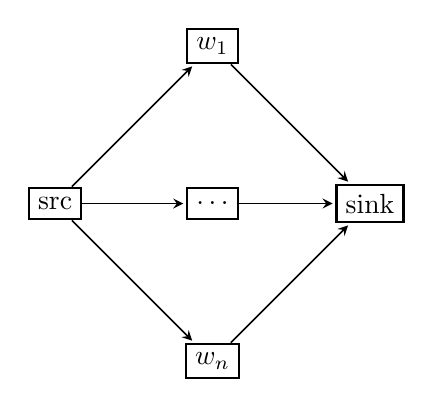
\begin{tikzpicture}[
     > = stealth, % arrow head style
     shorten > = 1pt, % don't touch arrow head to node
     auto,
     node distance = 2cm, % distance between nodes
     semithick % line style
 ]

 \tikzstyle{process} = [
     %cicrle,
     draw = black,
     thick,
     fill = white,
     minimum size = 4mm
 ]
 \tikzstyle{dots} = [
     draw = black,
     thick,
     fill = white,
     minimum size = 4mm
 ]

 \node[process] (src) {src};
 \node[dots] (wdots) [right of=src] {$\ldots$};
 \node[process] (wn) [below of=wdots] {$w_n$};
 \node[process] (w1) [above of =wdots] {$w_1$};
 \node[process] (sink) [right of=wdots] {sink};

 \path[->] (src) edge node {}(w1);
 \path[->] (src) edge node {}(wdots);
 \path[->] (src) edge node {}(wn);
 \path[->] (w1) edge node {}(sink);
 \path[->] (wdots) edge node {}(sink);
 \path[->] (wn) edge node {}(sink);
\end{tikzpicture}
}
	\caption{An example of data-parallelism exploiting the MacQueen gap.}
	\label{fig:data_parallel_kpn}
\end{figure}

This asynchronous execution can be used to execute multiple workers in a data-parallel fashion.
Figure~\ref{fig:data_parallel_kpn} shows an example of a network which does this.
The worker processes $w_1, \ldots, w_n$ can exploit data parallelism by dividing a workload into different parts.
This allows us to asynchronously execute the workloads, as long as we take care to preserve the order at the sink node. 
We can achieve this by making it part of the logic of the channels.
In~\cite{khasanov_parmaditam18} we proposed to exploit this gap and tested an implementation of this in \ac{MAPS}, which modified the FIFO libraries of nodes labeled as data-parallel to relax the deterministic semantics of the \ac{KMQ} blocking-reads and allowed asynchronous execution of data-parallel workers while preserving the deterministic \ac{KPN} execution.
The implementation of this library is beyond the contribution of this thesis, which is limited to the theoretical part of identifying the semantics gap and ways of exploiting it.   %parma_ditam, cgo_src (should I move this to applications?)

\chapter{Language-Level Transformations}
\section{Ohua}
This section reviews some programming languages and how they provide ``freedom from choice'' in the sense of A. Sangiovani-Vincentelli~\cite{lee2019freedom}.
There is a distinct sense in this is the central question of programming languages in general.
By removing memory management through having no pointer arithmetic and garbage collection, Java frees its users from multiple families of errors that are possible in C.
Rust's ownership types take a different approach, also removing complete families of memory-management based errors, without introducing large performance overheads or unpredictable behavior from the garbage collector.

These kinds of ``freedom from choice'' in general-purpose languages are beyond the scope of this thesis, which focuses on \acp{MoC} like those described in Chapter~\ref{chap:mocs}.
In well-defined \acp{MoC} like the ones discussed here, on the other hand, the temptation to break away from the semantics might be higher.
A very interesting observation and discussion of this phenomenon can be found in~\cite{tasharofi2013scala}, which shows not only that developers commonly break away from the semantics if they are not enforced, but also gives multiple explanations why.
This is why it is not advisable to expose these as a library, but rather as a full language, as much as possible. 
Here we will briefly survey languages focused on \ac{MoC}-based paradigms.

\subsection{Dataflow, Actors and Discrete Events}
\label{sec:general_dataflow_tools}

Most well-known languages that follow \acp{MoC} like the ones described here are based on the actor model.
Compared to more sophisticated models, the actor model has mostly intuitive semantics.
The Erlang language is a successful example of a language whose semantics are in principle an implementation of the (Hewitt-Agha) actor model.\index{Erlang}
The Rebeca language~\cite{sirjani2004formal}, which is primarily a design and specification language used in model checking, is also an actor-based language.\index{Rebeca}
Another prominent example is the CAL actor language~\cite{eker2003cal}, and has been used to define the \ac{RVC} standard~\cite{bhattacharyya2011overview}.
The \ac{RVC}-CAL compiler\footnote{\url{https://sourceforge.net/projects/orcc/}} is an Eclipse-based compiler for the CAL actor language which is used to compile the \ac{RVC} reference implementations.\index{\ac{RVC}-CAL}

Another prominent \ac{MoC}-based programming environment from academia is Ptolemy~II\cite{Ptolemaeus:14:SystemDesign}. 
In contrast to most of the other frameworks, Ptolemy~II supports a plethora of \ac{MoC}, including most of the models discussed in this thesis. 
Also in contrast to most other frameworks, \acp{MoC} are a central component of Ptolemy~II, which makes them explicit using \emph{directors}\index{Ptolemy~II}.
The framework uses the Java programming language to allow the definition of arbitrary actors, but it also comes with a large library of pre-defined actors.
Figure~\ref{fig:audio_filter_ptolemy} shows an implementation of an audio filter, which while not identical, is semantically similar to our running example described in Chapter~\ref{chap:mapping}.
This implementation uses only pre-defined actors in Ptolemy~II.

\begin{figure}[t]
	\centering
	\includegraphics[width=0.9\textwidth]{figures/audio_filter_ptolemy_screenshot.png}
	\caption{An audio filter in \ac{SDF} semantics in Ptolemy II}
	\label{fig:audio_filter_ptolemy}
	%	\vspace{-1mm}
\end{figure}

In the case of discrete-event models, there are many more well-established languages which implement them.
The hardware description languages VHDL and Verilog work with discrete-event semantics, since hardware does. 
The SystemC language, well known for discrete event simulations (of hardware), also has discrete event semantics~\cite{semantics_systemc}.
Finally, more on the software side are the Synchronous languages, like LUSTRE~\cite{lustre} or ESTEREL~\cite{esterel}, which are (complete) programming languages with a discrete event semantics.

Also in the discrete events domain is the Lingua Franca language~\cite{lohstroh_fdl20}\footnote{\url{https://github.com/icyphy/lingua-franca}}. 
Lingua Franca is a complex framework that implements the Reactors model, described in Section~ref{sec:rectors}.
This novel language is a self-described polyglot \emph{coordination language}, which means that it is not used to define the computation but rather to compose reactors written in a different language.
Similar to \ac{CPN}, nothing prevents programmers from ``cheating'' in the code of the reactors and going around the semantics, yet it does enforce them more strongly than a library, as it is a full \ac{DSL} that generates Reactors-based applications in a source-to-source compilation process.
Figure~\ref{fig:audio_filter_lf} shows the Lingua Franca programming environment with an implementation of the audio filter benchmark.
We will not discuss the framework more in detail, as the design and implementation of Lingua Franca is not part of the contribution of this thesis.

\begin{figure}[t]
	\centering
	\includegraphics[width=0.9\textwidth]{figures/audio_filter_lf_screenshot.png}
	\caption{The audio filter example in Lingua Franca}
	\label{fig:audio_filter_lf}
	%	\vspace{-1mm}
\end{figure}

In Chapter~\ref{chap:mapping} we discussed the \ac{CPN} language at length, as well as the \ac{MAPS} framework which is used to lower \ac{CPN} to different implementations in heterogeneous systems.
In contrast\footnote{As an extension of C, the \ac{CPN} language also does not fundamentally prevent programmers from breaking the semantics.}, e.g. the YAPI programming interface~\cite{yapi} defines process networks only as a runtime library and can be evaded just like Scala developers do with actor frameworks~\cite{tasharofi2013scala}.
The Sesame framework uses YAPI-based programs, e.g. derived from Compaan~\cite{stefanov2003deriving} for \ac{dse}\cite{pimentel2006systematic}.
Most of the software synthesis flows discussed in Section~\ref{sec:software_synthesis_flows} use the languages described here, e.g. TURNUS which uses CAL or SystemCoDesigner which is based on SystemC.
Other systems like DAARM or \mocasin do not use actual source code for the applications but rather application models for \ac{DSE}.


Most of the flows discussed above and in Section~\ref{sec:software_synthesis_flows} are academic and deal with more sophisticated models. 
Many ideas that seem good in academia do not hold up in a practical development environment, where the learning curve of the models and time-to-market considerations change the field.
It is therefore not surprising that the more sophisticated models have seen less adoption.
For example, the LabVIEW Communications System Design Suite restricts the LabVIEW language to a dataflow \ac{MoC}.
Matlab Simulink has a dataflow-like semantic with time triggering, thus closer to discrete event models.
On the discrete-events side 

\subsection{Implicit Dataflow}

The languages surveyed so far are explicit about their abstractions: Actors, Reactors or Processes are declared explicitly.
Similarly, channels describing the dataflow are made explicit either through channel declarations or through the connection of explicit ports.
A programmer writing in e.g. \ac{CPN} or Lingua Franca has to have a model of the network describing the application in their head (or in their \acs{IDE}).
Implicit abstractions, on the other hand, work by generating implicit models from linguistic constructs that don't exhibit their structure directly.

Implicit abstractions as we just defined them are ubiquitous in programming languages.
Again, objects in \ac{OOP} are an implicit abstraction for data encapsulation that is fundamentally similar to actors.
A thorough classification  of these implicit models is outside the scope of this thesis.
Instead, we will look closely at the Ohua programming paradigm~\cite{ertel_phdthesis}, which derives a dataflow execution from functional semantics.

The Ohua programming model by S. Ertel and others is a powerful model of implicit parallelism which can be used to express parallelism at a language level without explict costructions like threads and locks. 
\index{Ohua}
As stated above, the parallelism comes from lowering an Ohua program into a dataflow-based execution.
This model is not part of the original contribution of this thesis.
However, it is central to several distinct original contributions of the thesis, and we will introduce it as background material.

Ohua itself is a general paradigm that works on multiple language, and the framework has evolved over the years of its development.
The version of Ohua we will discuss here first is based on Clojure and Java, but the Ohua compiler and its principles work with many languages,
and rutimes also exist at different levels of development e.g. for Rust, Javascript or Go.
Ohua is best understood by diving directly into examples. Consider the code in Listing~\ref{listing:ohua_audio_filter}.

\begin{listing}
\begin{minted}[linenos]{Clojure}
 ;; TODO: add the audio filter solution code.
 (ns wav-transform.core
  (:gen-class)
  (:import WavTransform))

(defn -main
  "I don't do a whole lot ... yet."
  [& args]
  (WavTransform/fromFile "oxp.wav" "oxp-transformed.wav")) 
\end{minted}
\caption{The Audio Filter Example written in Ohua}
\label{listing:ohua_audio_filter}
\end{listing}

Listing~\ref{listig:ohua_audio_filter} is based on Clojure, a dialect of Lisp.
It implements the same example from Chapter~\ref{chap:mapping} (cf. Listing~\ref{listing:audio_filter} or Figure~\ref{fig:audio_filter_graph}), a two-channel audio filter.
Internally, the compiler transforms this code into a dataflow graph for execution.
As a \ac{MoC}, this can be embeded in the Dennis dataflow models discussed in Chapter~\ref{chap:mocs}.
We will discuss the semantics of these dataflow graphs in Section~\ref{sec:ohua_dataflow}.
\todo{discuss example}.

The example in Figure~\ref{fig:ohua_example} can be transformed into a dataflow graph for execution. We will discuss this further in Section~\ref{sec:ohua_dataflow}.
The main advantage of this transformation is that a dataflow graph exposes concurrency, which can be exploited e.g. in a parallel execution or for optimizing \ac{I/O}(cf. Section~\ref{sec:yauhau}).
This duality between code and dataflow graphs is a core concept behind Ohua.
The other central pilar of the Ohua design concept are stateful functions, an abstraction that encapsulates functions with state and side-effects in the context of their dataflow execution.
\index{Ohua ! stateful functions}

\subsection{Stateful Functions}
The functional programming community has made the distinction between \emph{pure} and \emph{impure} functions widespread.
A pure function is a function in the mathematical sense of the word: it receives a certain input and, deterministically, produces an output.
This could be as simple as negating a boolean value, or as complicated as inference with a gargantuan deep neural network.
The main point is that the entirety of the usage of a function is that it returns a value in a deterministic fashion from its inputs.

In most imperative languages, like C or Java, functions usually also have side-effects. Writing the output to the terminal, storing data in a global data structure or even reading data from a sensor in a \ac{CPS}, these are all examples of side effects.
A language that only allows pure functions is basically useless, since even printing the result of a computation is impure.
Time is also fundamentally part of a computation, as we have discussed in Chapter~\ref{chap:mocs}, as can be an interaction with the outside world in the form of sensing and actuation in \acp{CPS}.

Stateful functions are a special abstraction, where the concept of pure functions is extended to consider the state of the computation. 
While this excludes aspects like the time of the computation and side-effects like actuation, it is general enough to cover large classes of functions used in most software.
A stateful function is a function $f : a \rightarrow b$ and an abstract state $S$, where the execution of the function can be seen as dependent of the state, which it also modifyies.
In other words, we consider $f$ as a function:
\begin{align}
  f : a \times S \rightarrow b \times S \label{eqn:state_thread}
\end{align}

Pure functions can be seen as a special case of stateful functions, with a trivial state $S = \{*\}$.

\begin{listing}
\begin{minted}[]{Java}
public class ParseVariable{
  @defsfn
  public ParseVariable (ExpressionObject expr, SymbolTable table){
    symbols = expr.parse();
    table.write(symbols);
    return(object);
  }
}
\end{minted}
\caption{An example of a stateful function.}
\label{listing:stateful_function}
\end{listing}


Listing~\ref{listing:stateful_function} shows an example of a stateful function, written in Java, which is identified as such by the \texttt{@defsfn} annotation.
TODO: Discuss (or improve) the example. Admittedly, I'm a bit confused by this, does the state have to be explicit as an input?
By anotating a function as stateful and being able to reason about its state, we can ensure its semantics are preserved when transforming to a dataflow execution.
Traditionally, stateful functions in Ohua are explicitly annotated as such~\cite{ertel_pmam18}.

\subsection{Dataflow Execution}
\label{sec:ohua_dataflow}


Figure~\ref{fig:ohua_example_df} depicts this example as a dataflow graph.
\todo{discuss dataflow graph}.


Ohua

The Ohua framework is based on these two design principles, yet the implementation has constantly evolved since its original inception~\cite{ertel2014framework}.
The work we will present in this chapter played a role in Ohua's evolution.
For this reason, we will discuss the concrete language and transformations in the context they were developed, instead of the latest instantiation of Ohua.

The concepts of Ohua itself and the implementation of the compiler are beyond the scope of this thesis. 
The rest of this chapter will focus mostly on formalizing the semantics and defining semantics-preserving transformations. 
Note that is the joint contribution of a collaborative work with multiple co-authors in~\cite{goens_multiprog18,ertel_cc18,ertel_haskell19,ertel_haskellsup19}. 
\section{yauhau}
The infrastructure of large internet companies today relies to a great extent on microservice-based architectures~\cite{}.

Discuss~\cite{ertel_cc18}.

Focus on methods of semantic equivalence, only cite results.
 %cc_18
\section{smap?}
Discuss idea behind~\cite{ertel_haskell19}, not implementation.

Also discuss formalization in Category Theory~\cite{ertel_haskellsup19}


\chapter{Novel Semantics}
Software synthesis refers to a series of related methods, with the common goal of efficiently deploying software on a specific hardware architecture. While the aim of this thesis is to analyze structures and present methods that are general to software synthesis as a whole, in practice we will always work with concrete design flows. In this chapter we will introduce the concepts behind software synthesis and mappings in a concrete such flow, mapping KPN applications onto heterogeneous hardware. The flow can be seen in Figure~\ref{fig:sofware_synthesis_flow}, and is presented in detail in~\cite{castrillon_phd}.

As is general in Software Synthesis, the applications to be axecuted are represented with an abstract representation linked with a model of computation, Kahn Process Networks (KPNs). Similarly, the target archtiecture is assumed to be known at compile-time, and is models via an abstract architecture model. The KPN model has a property that allows to capture the abstract execution behavior in a trace that is independent of the execution target. Combining these application and architecture models, and using an execution trace, a simulation can be used to estimate the performance of a mapping - an assignment of physical execution and communication resources on the target architecture to the logical (abstract) components of the KPN application. In an iterative process, this estimations can be leveraged to determine a near-optimal mapping subject to objective goals (e.g. execution time, energy conspmution). Finally, a compiler can lower the KPN application to an executable that uses the selected mapping.

The rest of this chapter will explore the various models refered to in this flow, with precise mathematical definitions and a discussion of common design choices and goals in this flow.

\section{Kahn Process Networks}
\Blindtext[2]

\section{Models of Heterogeneous Architectures}
\Blindtext[2]
Briefly discuss MoA paper (Pelcat et al).

\section{Traces}
\Blindtext[2]


\section{Mappings}
\Blindtext[2]

\section{reactors}
So far we have discussed multiple \acp{MoC} with different extensions.
Most models we have focused on in this thesis are deterministic, which as explained in the introduction, is an important and useful property of a model's semantics.
We have how determinism in \acp{KPN} allows us to simulate and analyze their execution.
Without it, many concepts we have seen in chapters~\ref{chap:mapping,chap:mapping_structures,chap:mapping_applications} breaks down.

The models we have discussed neglect one important aspect, however; they neglect time.
Computation takes time~\cite{lee2009computing}, and this is a fundamental property of its semantics which is usually implicit.
Determinism as we have discussed it here means that the output of a computation is a deterministic function of its input.
This does not mean that the time it takes is deterministic, as we have studied in~\cite{goens_scopes17}.
Especially in the context of \acp{CPS} or real-time systems, the computation time is an essential part of the functional specification of an application.
In this section we discuss the Reactor model~\cite{lohstroh_dac19}, which aims be a deterministic \ac{MoC} with timed semantics.

Briefly discuss as idea and dwell more mathematical aspects in~\cite{Lohstroh_cyphy19} (my contribution). Be careful to delineate contributions here.
Should I write full formalization? Discuss Lean proof (probably not finished in time)
 %dac19,cyphy
\section{autosar}
The automotive domain is 

Only superficially discuss~\cite{menard_date20}, basic connection (my contribution). Cite some results, but explicitly as Christian's work. %dac20_autosar
\section{5G}
Here discuss~\cite{wittig_ict20}, and results (these I can discuss more freely as mostly my contribution)

Then make connection to reactors: determinsim, time semantics, adaptability.

Open question: adaptability (mutations) %ict + new

\chapter{Benchmarking and Beyond}
\section{level graphs}
The third category of inputs for \mocasin is \texttt{sdf3}, which uses the \ac{\SDFFF} framework~\cite{sdf3}.
This framework is based on \ac{TGFF}, adapted to the \ac{SDF} model of computation.
We will discuss \ac{SDF} more in detail in Chapter~\ref{chap:mocs}.
However, for the purposes of benchmarking as discussed here, both \ac{SDF} and task graphs can be considered as special cases of \ac{KPN}.
The random graph generation of the \ac{\SDFFF} framework allows multiple configurations on the types of graphs it generates, controlling the number of actors (processes) as well as the degree of connectivity in the graph, firing rates and execution times of the actors, or if the graph is acycilic.

Random benchmark generation has two main advantages over using fixed benchmarks. The first advantage is the amount of benchmarks, which is virtually unlimited with a random generation approach.
The second advantage is the control over the properties of the benchmarks.
Using \ac{\SDFFF} we can consider precisely what effect the properties of the graph have on the algorithms (e.g. its size, or connectivity), by generating benchmarks which have the desired parameters for the independent variable we are investigating.
The main disadvantage is obvious: random benchmarks are not as realistic as actual benchmarks.
It is not clear if we will find a graph like the one generated by \ac{\SDFFF} in a real-life application.

Since we have both the \ac{CPN} and the \ac{E3S} benchmarks, we will focus our evaluation on those.
Instead of discussing the graph generation in \ac{SDFFF}, we will discuss random benchmark generation from a different type of graph, \emph{level graphs}\index{level graph}\cite{goens_multiprog18}.
The main difference is that for the use-case for level graphs in~\cite{goens_multiprog18} we \textbf{do not} have better, realistic benchmark we can use instead.

The context for benchmark generation we will discuss here is in microservice-oriented architectures.
In large internet companies like Facebook or Twitter, the infrastructure of the architecture consists of multiple micro-services that depend on each other.
A crucial factor for optimal performance is the amount of \ac{I/O} calls these microservices make.
We will discuss the use case more in-depth in Chapter~\ref{chap:programming_languages}. 
In this section we will only focus on the benchmark generation.

The microservice-based infrastructures from large companies like Facebook or Twitter are the \acf{IP} of these companies and not in the public domain.
If we want to improve and compare a method for optimizing \ac{I/O} in Facebook's spam-fighting service~\cite{marlow2014haxl}, we cannot use a large representative benchmark sample from Facebook to test against their method.
Instead, we observe the general structure of the programs in their work and device a methodology for generating random benchmarks, with a method we call level graphs~\cite{goens_multiprog18}.

Figure~\ref{fig:level_graph} shows an example of a level graph. 

TODO: describe graph construction and briefly outline code generation.

\begin{figure*}[th]
	\centering
	\includegraphics[width=\textwidth]{figures/level-graph.pdf}
	\caption{An example of a Level Graph. Reproduced from Figure~1 of \cite{goens_multiprog18}.}
	\label{fig:histograms}
\end{figure*} %multiprog
\section{MAPL + ML representations?}
In the previous two sections we have discussed multiple benchmarks in two different classes: hand-written benchmarks and randomly generated benchmarks.
We have discussed the advantages and disadvantages of both.
Hand-written benchmarks cost many person-hours to write and maintain, and are usually very limited due to \ac{IP}.
Random benchmarks can overcome the scarcity of hand written ones at the cost of accuracy, they are less realistic and not as useful for assessing how well a method will perform on real use-cases.
There is a third approach that sits in-between the two above, to use machine learning to generate benchmarks with realistic properties.
This section discusses this approach and its limitations.

\subsection{Generative models}
\label{sec:generative}

\begin{figure*}[th]
	\centering
	\includegraphics[width=\textwidth]{figures/illustration_histograms_ideal.pdf}
	\caption{An illustration of generative models in the Fischer-Wald setting.}
	\label{fig:histograms}
\end{figure*}

Machine learning models that could generate benchmarks fall under the general term ``generative models''.
There are different classes of generative models, however:
%Let again $p$ be the probability density function describing the probability of a programmer writing a piece of code $\omega \in \Omega$.
\begin{enumerate}
\item \label{fischer-wald} A model in the \textbf{Fischer-Wald setting} is a machine learning model solving the problem of density estimation~\cite{vapnik}. This means finding a probability $p'(t,\alpha_0)$ in a set of probabilities $\{ p'(t,\alpha) \mid \alpha \in \Lambda \}$ parametrized by elements of the parameter set $\Lambda$,
  such that for the risk functional $R(\alpha) = \int -\log(p'(t,\alpha)) dp(t)$, the value of $R(\alpha_0)$ is minimal over all $\alpha \in \Lambda$.
\item \label{conditional-estimation} A \textbf{conditional estimation} model can again mean a solution to a few different problems in different settings. For a random variable $Y$ over code, it estimates either the joint distribution $X \times Y$ or one of the conditional probabilities $p(y \mid X = x)$ or $p(x \mid Y = y)$, where $X$ is the random variable representing a piece of code (i.e. $X(\omega) = \omega$, the identity on $\Omega$)~\cite{vapnik}.

\end{enumerate}

The models from (\ref{conditional-estimation}) are interesting problems on their own and will be discussed in Section~\ref{sec:outlook}.
The focus of this paper is the discussion of using solutions to (\ref{fischer-wald}) for benchmark generation.
This problem is the basis for generative models of code, and solutions to (\ref{conditional-estimation}) are based on or related to it as well.

\subsection{Potential Problems}
\label{sec:potential_problems}
Generative models learn to produce samples similar to those they have seen in the training data. They could then be leveraged to create arbitrarily large benchmark sets.
The problem with this is that, in the ideal case for the Fischer-Wald setting, the code produced by the generative model should be indistinguishable from the training data.
Concretely, it should be code that is also i.i.d. with respect to the (implicit) pdf of code.
If this training set is available, then it can be used instead of the synthesized benchmarks.
Figure~\ref{fig:histograms} illustrates this further.

The theoretical pdf depicted represents, again, the probability for a particular program to be written.
To the right the illustration represents a plausible histogram of the code actually present in a training set.
Underneath it, two additional histograms are depicted. To the right, in green, a histogram that is plausibly synthesized by a good generative model trained with the training set.
While it need not be identical to the training set, it should be similar if the generative model has been trained well.
To the left, a histogram is depicted that illustrates a very implausible generated set.
How should the generative model know of the unlikely cases it has not seen, and produce no synthetic code that would never be written by a human?
By the definition in (\ref{fischer-wald}), the closer the histograms are to the depicted pdf, the better are the generative model and training set.

In case we want a ``representative benchmark'', it is thus not clear that a generative model like this is useful.
The programs created by the generative model are i.i.d. with respect to some $p'(t) = p'(t,\alpha_0)$ that is different from $p$.
For estimating $E[\mathcal{P}]$ we get additional accuracy by increasing the number of samples $l$ we use to estimate it.
This additional accuracy, however, could be canceled out by the error in $p'$ (as quantified by, e.g. $R(\alpha_0)$).
Whether this is the case, of course, depends on the concrete problem and errors, and cannot be concluded generally.
We believe, however, that it is probably the case for most instances of the state-of-the-art in generative models of code.
It is likely that with the current state of generative models, where enough training data is present to train such a model, the raw data should be at least good enough, if not even better than synthetic data from the model.

For the other kinds of benchmark, the situation is less problematic.
If we have a filter to distinguish the types of programs, e.g. one based on vectors of features interesting for the use case, then we can use generative models with these filters to produce benchmark sets of the kinds ``representative coverage benchmark'' and perhaps in some cases even ``fuzzing benchmark'', if the generative models generalize well and are run long enough to produce enough data.


Summarize~\cite{goens_mapl19}.

\subsection{Models of Code}

Then only briefly motivate~\cite{brauckmann_cc20} and \cite{brauckmann_fdl20}.

 %mapl, cc20

\chapter{Related Work}
\input{tex/related/semantics.tex}

\chapter{Conclusions} 
Here will be the conclusions.

\appendix
\chapter{Groups and Inverse Semigroups}
\label{appendix:groups}
Group theory and inverse semigroups

\chapter{Metric Spaces and Low-Distortion Embeddings}
\label{appendix:metric}
Metric spaces and low-distortion embeddings.

\chapter{Denotational Semantics}
\label{appendix:semantics}
\input{tex/appendix/semantics.tex}

\bibliographystyle{abbrv}
\bibliography{thesis}

\listoffigures

\printindex

\chapter*{List of Acronyms}
%https://tex.stackexchange.com/questions/38558/how-to-pluralize-an-acronym-which-ends-in-s-correctly#38559
\begin{acronym}
  \acro{CPS}{Cyber-Physical Systems}
  \acro{MPSoC}{Multi-Processor System-on-Chip}
  \acro{KPN}{Kahn Process Network}
  \acro{DSE}{Design-Space Exploration}
  \acro{CFS}{Completely Fair Scheduler}
  \acro{poset}{partially-ordered set}
  \acro{NoC}{Network on Chip}
  \acro{ISA}{Instruction-Set Architecture}
\end{acronym}

\clearpage


\end{document}
